% !TEX TS-program = xelatex
% !TEX encoding = UTF-8
\documentclass[11pt]{book}


% PACKAGES
\usepackage{fontspec} % Font selection for XeLaTeX; see fontspec.pdf for documentation
% LetterSpace=1.2,
\defaultfontfeatures{WordSpace=1.1,Ligatures=TeX, Mapping=tex-text} % to support TeX conventions like ``---''
\usepackage{xunicode} % Unicode support for LaTeX character names (accents, European chars, etc)
%\usepackage{hyperref}
%\usepackage{glossaries}
\usepackage{polyglossia}
\usepackage{xltxtra} % Extra customizations for XeLaTeX
%\setsansfont{Deja Vu Sans}
%\setmonofont{Deja Vu Mono}
% other LaTeX packages.....
%\usepackage[total={12cm,21cm},top=2.8cm, left=4.5cm, headsep=1.1cm, footskip=1.5cm, footnotesep=1cm, xetex]{geometry}
%\usepackage[textwidth=11cm, height=20cm, includehead, headsep=1.1cm, footnotesep=1cm, xetex, footskip=1.7cm, left=14em]{geometry}

\usepackage[textwidth=11cm, textheight=18cm, includehead, headsep=1.1cm, footnotesep=.8cm, xetex, footskip=1cm, left=5.2cm]{geometry}
\usepackage[a4,width=17cm,height=24cm,center,cross,axes,color=blue,cam]{crop}

\usepackage{pdfpages}
\usepackage{todonotes}
\usepackage{circledsteps}


\usepackage{tikz}
\usepackage{color}
\usetikzlibrary{positioning}% To get more advanced positioning options
\usetikzlibrary{decorations.text}


\parskip1pt
\parindent1.5em
%%%%%%%%%%%%%%%%%%%%%%%%%%%%%%%%%%%%%%%%%%%%%%%%%%%%%%%%%%%%%%%
% customize the TOC
\usepackage{tocloft}
\renewcommand{\cftsecafterpnum}{\hspace*{0em}}
\renewcommand{\cftsubsecafterpnum}{\hspace*{0em}}
\renewcommand{\cftsubsubsecafterpnum}{\hspace*{0em}}
\renewcommand{\cftchapafterpnum}{\hspace*{0em}}

\renewcommand\cftloftitlefont{\englishfont} % optional

\makeatletter
\newcommand \mydotfill {\leavevmode \cleaders \hb@xt@ .8em{\hss .\hss }\hfill \kern \z@}
\makeatother
%%%%%%%%%%%%%%%%%%%%%%%%%%%%%%%%%%%%%%%%%%%%%%%%%%%%%%%%%%%%%%%


\usepackage[font={small,it}]{caption}

%%%%%%%%%%%%%%%%%%%%%%%%%%%%%%%%%%%%%%%%%%%%%%%%%%%%%%%%%%%%%%%
% bibliography
\usepackage{natbib}

% notesep below is for the sep between year and page num
\setcitestyle{authoryear, round, aysep={ },numbers,open={},close={},notesep={,\thinspace }}
% to modify the appearance of the label (SANDERSON 2009) in the bibliography (get rid of []s):
\makeatletter                         % Reference list option change
\renewcommand\@biblabel[1]{#1:}      %   from [1] to 1:
\makeatother      
% Title of biblio
%For book-classes: 
%\newcommand{\UnexpandableProtect}{}
\newcommand{\mycite}[1]{\citeauthor{#1} \citeyear{#1}}
\newcommand{\mycitep}[2]{\citeauthor{#1} \citeyear{#1}, #2}

% Finally! To hide the numbering in the Biblio 
\makeatletter
\renewcommand\@biblabel[1]{}
\makeatother

% to change indentation in the Bibliography
\usepackage{enumitem}
\makeatletter
\renewenvironment{thebibliography}[1]
     {\section{Secondary Sources and Editions\bigskip}%
     \fancyhead[CE]{}
     \fancyhead[CO]{}
     \@mkboth{header!}{header!}%
      \begin{enumerate}[label={[\arabic{enumi}]},itemindent=-2em,leftmargin=2em]
      \@openbib@code
      \sloppy
      \clubpenalty4000
      \@clubpenalty \clubpenalty
      \widowpenalty4000
      \sfcode`\.\@m}
     {\def\@noitemerr
       {\@latex@warning{Empty `thebibliography' environment}}%
      \end{enumerate}}
\makeatother
%%%%%%%%%%%%%%%%%%%%%%%%%%%%%%%%%%%%%%%%%%%%%%%%%%%%%%%%%%%%%%%



\newcommand{\corr}{corr.}
\newcommand{\conj}{conj.}
\newcommand{\om}{om.}
\newcommand{\acorr}{{\englishfont $^{\scriptscriptstyle ac}$}}
\newcommand{\pcorr}{{\englishfont $^{\scriptscriptstyle pc}$}}


%%%%%%%%%%%%%%%%%%%%%%%%%%%%%%%%%%%%%%%%%%%%%%%%%%%%%%%%%%%%%%%
%INDEX
\newcommand{\csindex}[1]{#1\index{#1}}
\newcommand{\csindexx}[2]{#1\index{#2@#1}}
\newcommand{\csindexxx}[3]{#1\index{#2@#3}}
\newcommand{\cskt}[2]{\skt{#1}\index{#2@\skt{#1}}}
\newcommand{\sktx}[1]{\skt{#1}\index{#1@\skt{#1}}}

\renewenvironment{theindex}
               {%\if@twocolumn
                  %\@restonecolfalse
                %\else
                  %\@restonecoltrue
                %\fi
%               \columnseprule \z@
                \columnseprule 0pt
%               \columnsep 35\p@
                \columnsep 35pt
%               \twocolumn[\@makeschapterhead{\indexname}]%
                \twocolumn[%\makeschapterhead{\indexname}
                \bigskip
                \bigskip
                \bigskip
                \bigskip

{\englishfont\Large\hfill\textit{General Index}\hfill}

 Sanskrit words, including titles of works, are typeset
 in \textit{italics}. Sanskrit names of deities, divine beings,
 humans (including authors), months, etc., and the
 names of modern authors, are written in a non-italic,
 standard typeface with capitalised initial letters.
 English words are presented in a non-italic, standard typeface.
 (The boundaries between these categories are sometimes fluid.)
\par \vskip 20pt]%
% Two lines below were the original.  I changed them so that the
% heading of the following pages would suit the previous chapters.
% But I am not certain if that was what Dominic and Haru wanted.
%                \markboth{\MakeUppercase\indexname}%
%                        {\MakeUppercase\indexname}%
              %  \markboth{Niśvāsatattvasaṃhitā}{Index to Introduction and Notes}
%               \thispagestyle{plain}\parindent\z@
                \thispagestyle{plain}\parindent0pt
%               \parskip\z@ \@plus .3\p@\relax
                \parskip0pt plus .3pt\relax
                \def\idxitem{\par\hangindent 40pt}
                \let\item\idxitem%
}
%              {\if@restonecol\onecolumn\else\clearpage\fi}
               {\onecolumn}
%%%%%%%%%%%%%%%%%%%%%%%%%%%%%%%%%%%%%%%%%%%%%%%%%%%%%%%%%%%%%%%





\tolerance=100
\hbadness=100
\hfuzz=2pt

% FONT STUFF
%\newfontfamily\devanagarifont[Script=Devanagari]{Sanskrit2003}
\newfontfamily\newarfont{Noto Sans Newa}
\usepackage[medium,lining,tabular]{ebgaramond}
\newfontfamily\devanagarifont[Scale=1,Script=Devanagari]{Sanskrit2003}
\newfontfamily\devanagarifontbold[Scale=1,Script=Devanagari]{Sanskrit2003}
%\newfontfamily\englishfont[Scale=1,Script=Latin]{EB Garamond}
\newcommand{\englishfont}{\ebgaramond}
%\newfontfamily\smallerfont[Scale=.9,Script=Latin]{EB Garamond}
\newcommand{\smallerfont}{\ebgaramond}

%\renewcommand{\baselinestretch}{.95}
% Activate to begin paragraphs with an empty line rather than an indent
%\usepackage[parfill]{parskip}
% support the \includegraphics command and options:
\usepackage{graphicx} 
\usepackage{makeidx}



%%%%%%%%%%%%%%%%%%%%%%%%%%%%%%%%%%%%%%%%%%%%%%%%%%%%%%%%%%%%%%%
%HEADER
\usepackage{fancyhdr}
\pagestyle{fancy}

\fancyhead[CE]{}
\fancyhead[CO]{}
\renewcommand{\headrulewidth}{0pt}
\fancyfoot[C]{\thepage}
\addtolength{\topmargin}{-2.49998pt}

%%%%%%%%%%%%%%%%%%%%%%%%%%%%%%%%%%%%%%%%%%%%%%%%%%%%%%%%%%%%%%%

%%%%%%%%%%%%%%%%%%%%%%%%%%%%%%%%%%%%%%%%%%%%%%%%%%%%%%%%%%%%%%%
% TOC

% this is to get rid of the page numbers on the pages of the toc
\fancypagestyle{plain}{%
  \fancyhf{}                          % clear all header and footer fields
  \renewcommand{\headrulewidth}{0pt}
  \renewcommand{\footrulewidth}{0pt}
}

% no section numbering in text:
\setcounter{secnumdepth}{0}
\setcounter{tocdepth}{3}

% section titles
\usepackage{titlesec}

  \titleformat{\chapter}%
  {\centering\normalfont\englishfont\Large\it}{%
    %\hspace*{-4.5em}\rule[-1.35mm]{4.5em}{1.25em}
    %{\color{white}\hspace{-1cm}\normalfont\thesection\hspace{5pt}}
  }{0em}{}

  % old color format I used to have:
%  \titleformat{\section}
%  {\normalfont\Large\itshape\color{red}}{%
%    \hspace*{-4.5em}\rule[-1.35mm]{4.5em}{1.25em}
%    {\color{white}\hspace{-1cm}\normalfont\thesection\hspace{5pt}}
%  }{0em}{}{}

%\titlespacing*{<command>}{<left>}{<before-sep>}{<after-sep>}
\titlespacing*{\section}
{0pt}{5.5ex plus 1ex minus .2ex}{.3em}

  \titleformat{\section}
  {\englishfont\large}{%
    {\englishfont\large\bf\thesection}  }{0em}{}{}


%\titlespacing*{<command>}{<left>}{<before-sep>}{<after-sep>}
\titlespacing*{\subsection}
{0pt}{2.5ex}{.3em}

  \titleformat{\subsection}
  {\normalfont\itshape}{%
    {\englishfont\itshape\thesection}
  }{0em}{}{}

 % \titleformat{\subsection}
 % {\normalfont\large\itshape\color{brown}}{%
 %   %\hspace*{-4.5em}\rule[-1.35mm]{4.5em}{1.25em}
    %{\color{white}\hspace{-1cm}\normalfont\thesubsection\hspace{5pt}}
 % }{0em}{}

  \titleformat{\subsubsection}
  {\normalfont}{%
   % \hspace*{-4.5em}\rule[-1.35mm]{4.5em}{1.25em}
   % {\color{white}\hspace{-1cm}\normalfont\thesubsection\hspace{5pt}}
  }{0em}{}
  
%\newcommand{\mychapter}[1]{\pagebreak\thispagestyle{empty}\ \vskip10em\begin{center}{\huge#1}\label{#2}\end{center}\vfill\pagebreak}
\newcommand{\mychapter}[1]{\chapter*{#1}%
        \addtocontents{toc}{\protect\contentsline{chapter}{\protect\numberline{\hspace{2em}}{\englishfont#1}}{}{}}}
\newcommand{\myblankchapter}[2]{\thispagestyle{empty}\ \vspace{10em}\\ \begin{center}{\Large#1}\end{center}\vfill%
        \addtocontents{toc}{\protect\contentsline{chapter}{\protect\numberline{\hspace{2em}}{\englishfont#2}}{}{}}}

%\newcommand{\mysection}[2]{\vskip1em\begin{center}{\textsc{\large #1}}\end{center}\label{#2}\vskip1em}
\newcommand{\mysection}[1]{\section{#1}
\addtocontents{toc}{\protect\contentsline{section}{\protect\numberline{}#1}{}}}


\newcommand{\mysubsection}[2]{\noindent\textit{#1}\label{#2}\\%
\noindent%
}
\newcommand{\mysubsubsection}[2]{\noindent{\color{black}{\textbf{#1}}}\label{#2}\hskip2em}
\newcommand{\msdescr}[2]{\medskip\noindent{\color{black}{\large\textbf{#1}}}\label{#2}\hskip2em}
%%%%%%%%%%%%%%%%%%%%%%%%%%%%%%%%%%%%%%%%%%%%%%%%%%%%%%%%%%%%%%%




%%%%%%%%%%%%%%%%%%%%%%%%%%%%%%%%%%%%%%%%%%%%%%%%%%%%%%%%%%%%%%%
% FOOTNOTES
%\renewcommand{\footnoterule}{}
\usepackage[]{footmisc}
% Here you can modify the spacing between the footnote number and the text of footnote; keep this value and \hangfootparindent value the same
\renewcommand{\footnotelayout}{\hspace{.5em}}
\renewcommand{\hangfootparindent}{\hspace{.5em}}

\newcommand\blankfootnote[1]{%
  \let\thefootnote\relax\footnotetext{#1}%
  \let\thefootnote\svthefootnote%
}

%%%%%%%%%%%%%%%%%%%%%%%%%%%%%%%%%%%%%%%%%%%%%%%%%%%%%%%%%%%%%%%




%MISC COMMANDS
\newcommand{\skt}[1]{\textit{#1}}
\newcommand{\ie}[1]{(\textit{#1})}
\newcommand{\skttitle}[2]{\textsl{#1}\index{#2@\textsl{#1}}}
\newcommand{\CHECK}{{\englishfont\color{red}{CHECK}}}
\newcommand{\uncl}[1]{${\wr}$#1${\wr}$}
%\newcommand{\shortsyllable}{\raise.15em\hbox{˘}}
\newcommand{\shortsyllable}{$\cup$}
\newcommand{\similar}{${\approx}$}
%\newcommand{\unmetr}{unmetr.}
\newcommand{\unmetr}{{\englishfont (unmetr.)}}
\newcommand{\compare}{{cf.}}
\newcommand{\asrama}{\cskt{āśrama}{asrama}}
\newcommand{\CE}{{\textsc{ce}}}
\newcommand{\BC}{{\textsc{bc}}}
\newcommand{\AD}{{\textsc{ad}}}
\newcommand{\fol}{f.\thinspace}
\newcommand{\fols}{ff.\thinspace}
\newcommand{\Fol}{F.\thinspace}
\newcommand{\Fols}{Ff.\thinspace}
\newcommand{\verbalroot}[1]{$\sqrt{#1}$}
\newcommand{\verify}{{\color{red}{CHECK}}}
\newcommand{\hide}[1]{}
\newcommand{\dbldanda}{||}
\newcommand{\il}{${\CHECK}$}
\newcommand{\lost}{\englishfont{×}}
\newcommand{\mutacumliquida}{\skt{krama} licence\index{krama licence@\skt{krama} licence}}
\newcommand{\krama}{\skt{krama}\index{krama licence@\skt{krama} licence}}
\newcommand{\stemform}{stem form\index{stem form (\skt{prātipadika})}}
\newcommand{\Stemform}{Stem form\index{stem form (\skt{prātipadika})}}

\newcommand{\recto}{$^r$}
\newcommand{\verso}{$^v$}

%SMALL CAPS HACKS
\newcommand\scR{r\kern-.35em\raisebox{-.17em}{.}\kern.15em}
\newcommand\scS{s\kern-.35em\raisebox{-.17em}{.}\kern.13em}
\newcommand\scM{m\kern-.5em\raisebox{-.17em}{.}\kern.25em}

% for the translation: chapter and verse number; translation; notes
\newcommand{\slokawithfn}[3]{\blankfootnote{\kern-1em#1: #3}%
%\textbf
\noindent{#1} #2\medskip}

\newcommand{\slokawithoutfn}[2]{%
%\textbf
\noindent{#1} #2\medskip}

\renewcommand{\labelitemi}{--}

% INPUT titles, authors, sigla
%% SANSKRIT WORKS
\newcommand{\AstangHr}{\textsl{A\-ṣṭā\-ṅga\-hṛ\-da\-ya}\index{Astangahrdaya@\textsl{Aṣṭāṅgahṛdaya}}}
\newcommand{\ASTANGHR}{AṣṭāṅgHṛ\index{Astangahrdaya@\textsl{Aṣṭāṅgahṛdaya}}}

\newcommand{\AgniP}{\textsl{A\-gni\-pu\-rā\-ṇa}\index{Agnipurana@\textsl{Agnipurāṇa}}}
\newcommand{\AGNIP}{AgniP\index{Agnipurana@\textsl{Agnipurāṇa}}}

\newcommand{\Amara}{\textsl{Amarakośa}\index{Amarakosa@\textsl{Amarakośa}}}
\newcommand{\AMARA}{Amara\index{Amarakosa@\textsl{Amarakośa}}}

\newcommand{\Uums}{\textsl{Utta\-ro\-tta\-ma\-ma\-hā\-saṃ\-vā\-da}\index{Uttarottaramahasamvada@\textsl{Uttarottaramahāsaṃvāda}}}
\newcommand{\UUMS}{UUMS\index{Uttarottaramahasamvada@\textsl{Uttarottaramahāsaṃvāda}}}

\newcommand{\Ums}{\textsl{Umāmaheśvarasaṃvāda}\index{Umamahesvarasamvada@\textsl{Umāmaheśvarasaṃvāda}}}
\newcommand{\UMS}{UMS\index{Umamahesvarasamvada@\textsl{Umāmaheśvarasaṃvāda}}}


\newcommand{\KurmP}{\textsl{Kū\-rma\-pu\-rā\-ṇa}\index{Kurmapurana@\textsl{Kūrmapurāṇa}}}
\newcommand{\KURMP}{KūrmP\index{Kurmapurana@\textsl{Kūrmapurāṇa}}}

\newcommand{\GautDhS}{\textsl{Gau\-ta\-ma\-dha\-rma\-sū\-tra}\index{Gautamadharmasutra@\textsl{Gautadharmasūtra}}}
\newcommand{\GAUTDHS}{GautDhS\index{Gautamadharmasutra@\textsl{Gautadharmasūtra}}}

\newcommand{\Caraka}{\textsl{Ca\-ra\-ka}\index{Caraka@\textsl{Caraka}}}
\newcommand{\CARAKA}{Caraka\index{Caraka@\textsl{Caraka}}}

\newcommand{\TakI}{\textsl{Tā\-ntri\-kā\-bhi\-dhā\-na\-ko\-śa I}\index{Tantrikabhidhanakosa@\textsl{Tāntrikābhidhānakośa}}}
\newcommand{\TAKI}{TAK I\index{Tantrikabhidhanakosa@\textsl{Tāntrikābhidhānakośa}}}

\newcommand{\TakII}{\textsl{Tā\-ntri\-kā\-bhi\-dhā\-na\-ko\-śa II}\index{Tantrikabhidhanakosa@\textsl{Tāntrikābhidhānakośa}}}
\newcommand{\TAKII}{TAK II\index{Tantrikabhidhanakosa@\textsl{Tāntrikābhidhānakośa}}}

\newcommand{\TakIII}{\textsl{Tā\-ntri\-kā\-bhi\-dhā\-na\-ko\-śa III}\index{Tantrikabhidhanakosa@\textsl{Tāntrikābhidhānakośa}}}
\newcommand{\TAKIII}{TAK III\index{Tantrikabhidhanakosa@\textsl{Tāntrikābhidhānakośa}}}

\newcommand{\Diksottara}{\textsl{Dī\-kṣo\-tta\-ra}\index{Diksottara@\textsl{Dīkṣottara}}}
\newcommand{\DIKSOTTARA}{DīkṣU\index{Diksottara@\textsl{Dīkṣottara}}}

\newcommand{\Divyav}{\textsl{Di\-vyā\-va\-dā\-na}\index{Divyavadana@\textsl{Divyāvadāna}}}
\newcommand{\DIVYAV}{Divyāv\index{Divyavadana@\textsl{Divyāvadāna}}}

\newcommand{\DharmP}{\textsl{Dha\-rma\-pu\-tri\-kā}\index{Dharmaputrika@\textsl{Dharmaputrikā}}}
\newcommand{\DHARMP}{DharmP\index{Dharmaputrika@\textsl{Dharmaputrikā}}}

\newcommand{\NaradaP}{\textsl{Nā\-ra\-da\-pu\-rā\-ṇa}\index{Naradapurana@\textsl{Nāradapurāṇa}}}
\newcommand{\NARADAP}{NāradaP\index{Naradapurana@\textsl{Nāradapurāṇa}}}

\newcommand{\Nisv}{\textsl{Ni\-śvā\-sa\-tattva\-saṃhi\-tā}\index{Nisvasatattvasamhita@\textsl{Niśvāsatattva\-saṃhitā}}}
\newcommand{\NISV}{Niśv\index{Nisvasatattvasamhita@\textsl{Niśvāsatattva\-saṃhitā}}}

\newcommand{\Nisvmukh}{\textsl{Ni\-śvā\-sa mu\-kha}\index{Nisvasamukha@\textsl{Niśvāsa mukha}}}
\newcommand{\NISVMUKH}{NiśvMukha\index{Nisvasamukha@\textsl{Niśvāsa mukha}}}

\newcommand{\Nisvmul}{\textsl{Ni\-śvā\-sa mū\-la}\index{Nisvasamula@\textsl{Niśvāsa mūla}}}
\newcommand{\NISVMUL}{NiśvMūl\index{Nisvasamukha@\textsl{Niśvāsa mūla}}}

\newcommand{\Nisvnaya}{\textsl{Ni\-śvā\-sa na\-ya}\index{Nisvasanaya@\textsl{Niśvāsa naya}}}
\newcommand{\NISVNAYA}{NiśvNaya\index{Nisvasamukha@\textsl{Niśvāsa naya}}}

\newcommand{\Nisvuttara}{\textsl{Ni\-śvā\-sa u\-tta\-ra}\index{Nisvasauttara@\textsl{Niśvāsa uttara}}}
\newcommand{\NISVUTTARA}{NiśvUttara\index{Nisvasauttara@\textsl{Niśvāsa uttara}}}

\newcommand{\NisvK}{\textsl{Ni\-śvā\-sa kā\-ri\-kā}\index{Nisvasakarika@\textsl{Niśvāsa kārikā}}}
\newcommand{\NISVK}{NiśvK\index{Nisvasakarika@\textsl{Niśvāsa kārikā}}}

\newcommand{\Padmap}{\textsl{Padma\-pu\-rā\-ṇa}\index{Padmapurana@\textsl{Padmapurāṇa}}}
\newcommand{\PADMAP}{PadmaP\index{Padmapurana@\textsl{Padmapurāṇa}}}

\newcommand{\Buddhacarita}{\textsl{Bu\-ddha\-ca\-ri\-ta}\index{Buddhacarita@\textsl{Buddhacarita}}}
\newcommand{\BUDDHACARITA}{BuddhCar\index{Buddhacarita@\textsl{Buddhacarita}}}

\newcommand{\BrahmaP}{\textsl{Bra\-hma\-pu\-rā\-ṇa}\index{Brahmapurana@\textsl{Brahmapurāṇa}}}
\newcommand{\BRAHMAP}{BrahmaP\index{Brahmapurana@\textsl{Brahmapurāṇa}}}

\newcommand{\BraYa}{\textsl{Bra\-hma\-yā\-ma\-la}\index{Brahmayamala@\textsl{Brahmayāmala}}}
\newcommand{\BRAYA}{BraYā\index{Brahmayamala@\textsl{Brahmayāmala}}}

\newcommand{\BrahmaVP}{\textsl{Bra\-hma\-vai\-va\-rta\-pu\-rā\-ṇa}\index{Brahmavaivartapurana@\textsl{Brahma\-vaivarta\-purāṇa}}}
\newcommand{\BRAHMAVP}{BrahmaVP\index{Brahmavaivartapurana@\textsl{Brahma\-vaivarta\-purāṇa}}}

\newcommand{\BhG}{\textsl{Bha\-ga\-va\-dgī\-tā}\index{Bhagavadgita@\textsl{Bhagavadgītā}}}
\newcommand{\BHG}{BhG\index{Bhagavadgita@\textsl{Bhagavadgītā}}}


\newcommand{\BhelaS}{\textsl{Bhe\-la\-saṃ\-hi\-tā}\index{Bhelasamhita@\textsl{Bhelasaṃhitā}}}
\newcommand{\BHELAS}{BhelaS\index{Bhelasamhita@\textsl{Bhelasaṃhitā}}}

\newcommand{\MBh}{\textsl{Mahābhārata}\index{Mahabharata@\textsl{Mahābhārata}}}
\newcommand{\MBH}{MBh\index{Mahabharata@\textsl{Mahābhārata}}}

\newcommand{\MahaSubhS}{\textsl{Ma\-hā\-su\-bhā\-ṣi\-ta\-saṃ\-gra\-ha}\index{Mahasubhasitasamgraha@\textsl{Mahā\-subhāṣita\-saṃgraha}}}
\newcommand{\MAHASUBHS}{MahāSubhS\index{Mahasubhasitasamgraha@\textsl{Mahā\-subhāṣita\-saṃgraha}}}

\newcommand{\MarkP}{\textsl{Mārkaṇḍeyapurāṇa}\index{Markandeyapurana@\textsl{Mārkaṇḍeyapurāṇa}}}
\newcommand{\MARKP}{MarkP\index{Markandeyapurana@\textsl{Mārkaṇḍeyapurāṇa}}}

\newcommand{\MatsP}{\textsl{Matsyapurāṇa}\index{Matsyapurana@\textsl{Matsyapurāṇa}}}
\newcommand{\MATSP}{MatsP\index{Matsyapurana@\textsl{Matsyapurāṇa}}}

\newcommand{\Mitaksara}{\textsl{Mi\-tā\-kṣa\-ra}\index{Mitaksara@\textsl{Mitākṣara}}}
\newcommand{\MITAKSARA}{Mitākṣara\index{Mitaksara@\textsl{Mitākṣara}}}

\newcommand{\Manu}{Manu\index{Manu@\textsl{Mānavadharmaśāstra}}}
\newcommand{\MANU}{Manu\index{Manu@\textsl{Mānavadharmaśāstra}}}

\newcommand{\BrahmandaPur}{\textsl{Bra\-hmā\-ṇḍa\-pu\-rā\-ṇa}\index{Brahmandapurana@\textsl{Brahmāṇḍapurāṇa}}}
\newcommand{\BRAHMANDAPUR}{BrahmāṇḍaP\index{Brahmandapurana@\textsl{Brahmāṇḍapurāṇa}}}

\newcommand{\BhavP}{\textsl{Bha\-vi\-ṣya\-pu\-rā\-ṇa}\index{Bhavisyapurana@\textsl{Bhaviṣyapurāṇa}}}
\newcommand{\BHAVP}{BhavP\index{Bhavisyapurana@\textsl{Bhaviṣyapurāṇa}}}

\newcommand{\BhagP}{\textsl{Bhā\-ga\-va\-ta\-pu\-rā\-ṇa}\index{Bhagavatapurana@\textsl{Bhāgavatapurāṇa}}}
\newcommand{\BHAGP}{BhāgP\index{Bhagavatapurana@\textsl{Bhāgavatapurāṇa}}}

\newcommand{\YajnS}{\textsl{Yājñavalkyasmṛti}\index{Yajnavalkyasmrti@\textsl{Yājñavalkyasmṛti}}}
\newcommand{\YAJNS}{YājñS\index{Yajnavalkyasmrti@\textsl{Yājñavalkyasmṛti}}}

\newcommand{\LinPu}{\textsl{Li\-ṅga\-pu\-rā\-ṇa}\index{Lingapurana@\textsl{Liṅgapurāṇa}}}
\newcommand{\LINPU}{LiṅP\index{Sivapurana@\textsl{Śivapurāṇa}}}

\newcommand{\Ramayana}{\textsl{Rā\-mā\-ya\-ṇa}\index{Ramayana@\textsl{Rāmāyaṇā}}}
\newcommand{\RAMAYANA}{\textsl{Rāmāyaṇa}\index{Ramayana@\textsl{Rāmāyaṇā}}}

\newcommand{\Vagmati}{\textsl{Vā\-gma\-tī\-māhātmya\-praśaṃsā}\index{Vagmatimahatmyaprasamsa@\textsl{Vāgmatīmāhātmyapraśaṃsā}}}
\newcommand{\VAGMATI}{VāgMāPr\index{Vagmatimahatmyaprasamsa@\textsl{Vāgmatīmāhātmyapraśaṃsā}}}

\newcommand{\VisnuP}{\textsl{Vi\-ṣṇu\-pu\-rā\-ṇa}\index{Visnupurana@\textsl{Viṣṇupurāṇa}}}
\newcommand{\VISNUP}{ViṣṇuP\index{Visnupurana@\textsl{Viṣṇupurāṇa}}}

\newcommand{\VDhU}{\textsl{Vi\-ṣṇu\-dha\-rmo\-tta\-ra}\index{Visnudharmottara@\textsl{Viṣṇudharmottara}}}
\newcommand{\VDHU}{VDhU\index{Visnudharmottara@\textsl{Viṣṇudharmottara}}}

\newcommand{\VamP}{\textsl{Vā\-ma\-na\-pu\-rā\-ṇa}\index{Vamanapurana@\textsl{Vāmanapurāṇa}}}
\newcommand{\VAMP}{VarP\index{Vamanapurana@\textsl{Vāmanapurāṇa}}}

\newcommand{\VayuP}{\textsl{Vā\-yu\-pu\-rā\-ṇa}\index{Vayupurana@\textsl{Vāyupurāṇa}}}
\newcommand{\VAYUP}{VāyuP\index{Vayupurana@\textsl{Vāyupurāṇa}}}

\newcommand{\VarP}{\textsl{Va\-rā\-ha\-pu\-rā\-ṇa}\index{Varahapurana@\textsl{Varāhapurāṇa}}}
\newcommand{\VARP}{VarP\index{Varahapurana@\textsl{Varāhapurāṇa}}}

\newcommand{\VasDh}{\textsl{Vā\-si\-ṣṭha\-dha\-rma\-śā\-stra}\index{Vasisthadharmasastra@\textsl{Vāsiṣṭhadharmaśāstra}}}
\newcommand{\VASDH}{VasDh\index{Vasisthadharmasastra@\textsl{Vāsiṣṭhadharmaśāstra}}}

\newcommand{\VDh}{\textsl{Vi\-ṣṇu\-dha\-rma}\index{Visnudharma@\textsl{Viṣṇudharma}}}
\newcommand{\VDH}{VDh\index{Visnudharma@\textsl{Viṣṇudharma}}}

\newcommand{\VisnuS}{\textsl{Vi\-ṣṇu\-smṛ\-ti}\index{Visnusmrti@\textsl{Viṣṇusmṛti}}}
\newcommand{\VISNUS}{ViṣṇuS\index{Visnusmrti@\textsl{Viṣṇusmṛti}}}

\newcommand{\SivPu}{\textsl{Śi\-va\-pu\-rā\-ṇa}\index{Sivapurana@\textsl{Śivapurāṇa}}}
\newcommand{\SIVPU}{ŚivP\index{Sivapurana@\textsl{Śivapurāṇa}}}

\newcommand{\Vss}{\textsl{Vṛ\-ṣa\-sā\-ra\-saṃ\-gra\-ha}\index{Vrsasarasamgraha@\textsl{Vṛṣasārasaṃgraha}}}
\newcommand{\Vsssc}{{V\scR\scS a\-sā\-ra\-sa\scM\-gra\-ha}%
								\index{Vrsasarasamgraha@\textsl{Vṛṣasārasaṃgraha}}}
\newcommand{\VSS}{{VSS}\index{Vrsasarasamgraha@\textsl{Vṛṣasārasaṃgraha}}}

\newcommand{\SivP}{\textsl{Śivapurāṇa}\index{Sivapurana@\textsl{Śivapurāṇa}}}
\newcommand{\SIVP}{SivP\index{Sivapurana@\textsl{Śivapurāṇa}}}

\newcommand{\SDhS}{\textsl{Śi\-va\-dhar\-ma\-śās\-tra}\index{Sivadharmasastra@\textsl{Śivadharmaśāstra}}}
\newcommand{\SDHS}{ŚDhŚ\index{Sivadharmasastra@\textsl{Śivadharmaśāstra}}}

\newcommand{\SDhSangr}{\textsl{Śi\-va\-dhar\-ma\-saṅ\-gra\-ha}\index{Sivadharmasangraha@\textsl{Śivadharmasaṅgraha}}}
\newcommand{\SDHSANGR}{ŚDhSaṅgr\index{Sivadharmasangraha@\textsl{Śivadharmasaṅgraha}}}

\newcommand{\SDhU}{\textsl{Śi\-va\-dhar\-mo\-tta\-ra}\index{Sivadharmottara@\textsl{Śivadharmottara}}}
\newcommand{\SDHU}{ŚDhU\index{Sivadharmottara@\textsl{Śivadharmottara}}}

\newcommand{\SannyasUp}{\textsl{Sa\-nnyā\-so\-pa\-ni\-ṣad}\index{Sannyasopanisad@\textsl{Sanyāsopaniṣad}}}
\newcommand{\SANNYASUP}{SannyāsUp\index{Sannyasopanisad@\textsl{Sanyāsopaniṣad}}}

\newcommand{\SkandaP}{\textsl{Ska\-nda\-pu\-rā\-ṇa}\index{Skandapurana@\textsl{Skandapurāṇa}}}
\newcommand{\SKANDAP}{SkandaP\index{Skandapurana@\textsl{Skandapurāṇa}}}

\newcommand{\Hyp}{\textsl{Ha\-ṭha\-yo\-ga\-pra\-dī\-pi\-kā}\index{Hathayogapradipika@\textsl{Haṭhayogapradīpikā}}}
\newcommand{\HYP}{HYP\index{Hathayogapradipika@\textsl{Haṭhayogapradīpikā}}}



\newcommand{\titleface}[1]{\textit{#1}}

% SANSKRIT WORKS
\newcommand{\Arthasastra}{\titleface{A\-rtha\-śā\-stra}\index{Arthasastra@\titleface{Artha\-śāstra}}}

\newcommand{\AgamaKL}{\titleface{Ā\-ga\-ma\-ka\-lpa\-la\-tā}\index{Agamakalpalata@\titleface{Āgama\-kalpa\-latā}}}
\newcommand{\AGAMAKL}{ĀgamaKL\index{Agamakalpalata@\titleface{Āgama\-kalpa\-latā}}}

\newcommand{\Apastambadharmasutra}{\titleface{Ā\-pa\-sta\-mba\-dharma\-sūtra}\index{Apastambadharmasutra@\titleface{Ā\-pa\-sta\-mba\-dharma\-sūtra}}}
\newcommand{\APASTDHSU}{ĀpastDhSū\index{Apastambadharmasutra @\titleface{Ā\-pa\-sta\-mba\-dharma\-sūtra}}}

\newcommand{\AstangHr}{\titleface{A\-ṣṭā\-ṅga\-hṛ\-da\-ya}\index{Astangahrdaya@\titleface{Aṣṭāṅgahṛdaya}}}
\newcommand{\ASTANGHR}{AṣṭāṅgHṛ\index{Astangahrdaya@\titleface{Aṣṭāṅgahṛdaya}}}

\newcommand{\AgniP}{\titleface{A\-gni\-pu\-rā\-ṇa}\index{Agnipurana@\titleface{Agnipurāṇa}}}
\newcommand{\AGNIP}{AgniP\index{Agnipurana@\titleface{Agnipurāṇa}}}

\newcommand{\Amara}{\titleface{Amarakośa}\index{Amarakosa@\titleface{Amarakośa}}}
\newcommand{\AMARA}{Amara\index{Amarakosa@\titleface{Amarakośa}}}

\newcommand{\Isanasiva}{\titleface{Īśāna\-śiva\-guru\-deva\-paddhati}\index{Isanasivagurudevapaddhati@\titleface{Īśāna\-śiva\-guru\-deva\-paddhati}}}
\newcommand{\ISGDP}{\titleface{ĪŚGDP}\index{Isanasivagurudevapaddhati@\titleface{Īśāna\-śiva\-guru\-deva\-paddhati}}}

\newcommand{\Uums}{\titleface{Utta\-ro\-tta\-ra\-ma\-hā\-saṃ\-vā\-da}\index{Uttarottaramahasamvada@\titleface{Uttarottaramahāsaṃvāda}}}
\newcommand{\UUMS}{UUMS\index{Uttarottaramahasamvada@\titleface{Uttarottaramahāsaṃvāda}}}

\newcommand{\Ums}{\titleface{Umā\-mahe\-śva\-ra\-saṃ\-vāda}\index{Umamahesvarasamvada@\titleface{Umāmaheśvarasaṃvāda}}}
\newcommand{\UMS}{UMS\index{Umamahesvarasamvada@\titleface{Umāmaheśvarasaṃvāda}}}


\newcommand{\RV}{ṚV\index{Rgveda@\titleface{Ṛgveda}}}

\newcommand{\KurmP}{\titleface{Kū\-rma\-pu\-rā\-ṇa}\index{Kurmapurana@\titleface{Kūrmapurāṇa}}}
\newcommand{\KURMP}{KūP\index{Kurmapurana@\titleface{Kūrmapurāṇa}}}

\newcommand{\GautDhS}{\titleface{Gau\-ta\-ma\-dha\-rma\-sū\-tra}\index{Gautamadharmasutra@\titleface{Gautamadharmasūtra}}}
\newcommand{\GAUTDHS}{GautDhS\index{Gautamadharmasutra@\titleface{Gautamadharmasūtra}}}

\newcommand{\Caraka}{\titleface{Ca\-ra\-ka\-saṃ\-hitā}\index{Carakasamhita@\titleface{Caraka\-saṃhitā}}}
\newcommand{\CARAKA}{Caraka\index{Carakasamhita@\titleface{Caraka\-saṃhitā}}}

\newcommand{\Jativiveka}{\titleface{Jā\-ti\-vi\-ve\-ka}\index{Jativiveka@\titleface{Jā\-ti\-vi\-ve\-ka}}}

\newcommand{\JayadRY}{\titleface{Ja\-ya\-dra\-tha\-yā\-yā\-ma\-la}\index{Jayadrathayamala@\titleface{Ja\-ya\-dra\-tha\-yā\-yā\-ma\-la}}}
\newcommand{\JRY}{JRY\index{Jayadrathayamala@\titleface{Ja\-ya\-dra\-tha\-yā\-yā\-ma\-la}}}

\newcommand{\TakI}{\titleface{Tā\-ntri\-kā\-bhi\-dhā\-na\-ko\-śa I}\index{Tantrikabhidhanakosa@\titleface{Tāntrikābhidhānakośa}}}
\newcommand{\TAKI}{TAK I\index{Tantrikabhidhanakosa@\titleface{Tāntrikābhidhānakośa}}}

\newcommand{\TakII}{\titleface{Tā\-ntri\-kā\-bhi\-dhā\-na\-ko\-śa II}\index{Tantrikabhidhanakosa@\titleface{Tāntrikābhidhānakośa}}}
\newcommand{\TAKII}{TAK II\index{Tantrikabhidhanakosa@\titleface{Tāntrikābhidhānakośa}}}

\newcommand{\TakIII}{\titleface{Tā\-ntri\-kā\-bhi\-dhā\-na\-ko\-śa III}\index{Tantrikabhidhanakosa@\titleface{Tāntrikābhidhānakośa}}}
\newcommand{\TAKIII}{TAK III\index{Tantrikabhidhanakosa@\titleface{Tāntrikābhidhānakośa}}}

\newcommand{\TakIV}{\titleface{Tā\-ntri\-kā\-bhi\-dhā\-na\-ko\-śa IV}\index{Tantrikabhidhanakosa@\titleface{Tāntrikābhidhānakośa}}}
\newcommand{\TAKIV}{TAK IV\index{Tantrikabhidhanakosa@\titleface{Tāntrikābhidhānakośa}}}

\newcommand{\Diksottara}{\titleface{Dī\-kṣo\-tta\-ra}\index{Diksottara@\titleface{Dīkṣottara}}}
\newcommand{\DIKSOTTARA}{DīkṣU\index{Diksottara@\titleface{Dīkṣottara}}}

\newcommand{\DivyAv}{\titleface{Di\-vyā\-va\-dā\-na}\index{Divyavadana@\titleface{Divyāvadāna}}}
\newcommand{\DIVYAV}{Divyāv\index{Divyavadana@\titleface{Divyāvadāna}}}

\newcommand{\DeviP}{\titleface{De\-vī\-pu\-rā\-ṇa}\index{Devipurana@\titleface{Devī\-purāṇa}}}
\newcommand{\DEVIP}{DevīP\index{Devipurana@\titleface{Devī\-purāṇa}}}

\newcommand{\DeviBh}{\titleface{De\-vī\-bhā\-ga\-vata}\index{Devibhagavata@\titleface{Devī\-bhāgavata}}}
\newcommand{\DEVIBH}{DevīBh\index{Devibhagavata@\titleface{Devī\-bhāgavata}}}

\newcommand{\DharmP}{\titleface{Dha\-rma\-pu\-tri\-kā}\index{Dharmaputrika@\titleface{Dharmaputrikā}}}
\newcommand{\DHARMP}{DharmP\index{Dharmaputrika@\titleface{Dharmaputrikā}}}

\newcommand{\Dharmasamuccaya}{\titleface{Dha\-rma\-samu\-cca\-ya}\index{Dharmasamuccaya@\titleface{Dharmasamuccaya}}}


\newcommand{\NaradaP}{\titleface{Nā\-ra\-da\-pu\-rā\-ṇa}\index{Naradapurana@\titleface{Nāradapurāṇa}}}
\newcommand{\NARADAP}{NāradaP\index{Naradapurana@\titleface{Nāradapurāṇa}}}

\newcommand{\NaradaParivr}{\titleface{Nāradaparivrājakopaniṣad}\index{Naradaparivrajakopanisad@\titleface{Nārada\-pari\-vrājako\-paniṣad}}}
\newcommand{\NARADAPARIVR}{NāradParivrUp\index{Naradaparivrajakopanisad@\titleface{Nārada\-pari\-vrājako\-paniṣad}}}

\newcommand{\Nisv}{\titleface{Ni\-śvā\-sa\-tattva\-saṃhi\-tā}\index{Nisvasatattvasamhita@\titleface{Niśvāsatattva\-saṃhitā}}}
\newcommand{\NISV}{Niśv\index{Nisvasatattvasamhita@\titleface{Niśvāsatattva\-saṃhitā}}}

\newcommand{\NisvMukha}{\titleface{Ni\-śvā\-sa mu\-khasūtra}\index{Nisvasatattvasamhita@\titleface{Niśvāsatattva\-saṃhitā}!\titleface{mukhasūtra}}}
\newcommand{\NISVMUKHA}{NiśvMukha\index{Nisvasatattvasamhita@\titleface{Niśvāsatattva\-saṃhitā}!\titleface{mukhasūtra}}}

\newcommand{\NisvMula}{\titleface{Ni\-śvā\-sa mū\-lasūtra}\index{Nisvasatattvasamhita@\titleface{Niśvāsatattva\-saṃhitā}!\titleface{mūlasūtra}}}
\newcommand{\NISVMULA}{NiśvMūl\index{Nisvasatattvasamhita@\titleface{Niśvāsatattva\-saṃhitā}!\titleface{mūlasūtra}}}

\newcommand{\NisvNaya}{\titleface{Ni\-śvā\-sa na\-yasūtra}\index{Nisvasatattvasamhita@\titleface{Niśvāsatattva\-saṃhitā}!\titleface{nayasūtra}}}
\newcommand{\NISVNAYA}{NiśvNaya\index{Nisvasatattvasamhita@\titleface{Niśvāsatattva\-saṃhitā}!\titleface{nayasūtra}}}

\newcommand{\NisvUttara}{\titleface{Ni\-śvā\-sa utta\-rasūtra}\index{Nisvasatattvasamhita@\titleface{Niśvāsatattva\-saṃhitā}!\titleface{uttarasūtra}}}
\newcommand{\NISVUTTARA}{NiśvUttara\index{Nisvasatattvasamhita@\titleface{Niśvāsatattva\-saṃhitā}!\titleface{uttarasūtra}}}

\newcommand{\NisvGuhya}{\titleface{Ni\-śvā\-sa gu\-hyasūtra}\index{Nisvasatattvasamhita@\titleface{Niśvāsatattva\-saṃhitā}!\titleface{guhyasūtra}}}
\newcommand{\NISVGUHYA}{NiśvGuhya\index{Nisvasatattvasamhita@\titleface{Niśvāsatattva\-saṃhitā}!\titleface{guhyasūtra}}}

\newcommand{\NisvK}{\titleface{Ni\-śvā\-sa kā\-ri\-kā}\index{Nisvasakarika@\titleface{Niśvāsakārikā}}}
\newcommand{\NISVK}{NiśvK\index{Nisvasakarika@\titleface{Niśvāsakārikā}}}

\newcommand{\NepMah}{\titleface{Nepāla\-mā\-hā\-tmya}\index{Nepalamahatmya@\titleface{Nepāla\-māhātmya}}}
\newcommand{\NEPMAH}{NepMā\index{Nepalamahatmya@\titleface{Nepāla\-māhātmya}}}

\newcommand{\Patimokkha}{\titleface{Pāti\-mokkha}\index{Patimokkha@\titleface{Pāti\-mokkha}}}
\newcommand{\PATMOKHA}{Pātimokkha\index{Patimokkha@\titleface{Pāti\-mokkha}}}

\newcommand{\PadmaP}{\titleface{Padma\-pu\-rā\-ṇa}\index{Padmapurana@\titleface{Padmapurāṇa}}}
\newcommand{\PADMAP}{PadmaP\index{Padmapurana@\titleface{Padmapurāṇa}}}

\newcommand{\ParasaraS}{\titleface{Pa\-rā\-śa\-ra\-smṛ\-ti}\index{Parasarasmrti@\titleface{Pa\-rā\-śa\-ra\-smṛ\-ti}}}

\newcommand{\PadmaS}{\titleface{Padma\-saṃ\-hi\-tā}\index{Padmasamhita@\titleface{Padma\-saṃhitā}}}
\newcommand{\PADMAS}{PadmaS\index{Padmasamhita@\titleface{Padma\-saṃhitā}}}

\newcommand{\Buddhacarita}{\titleface{Bu\-ddha\-ca\-ri\-ta}\index{Buddhacarita@\titleface{Buddhacarita}}}
\newcommand{\BUDDHACARITA}{BuddhCar\index{Buddhacarita@\titleface{Buddhacarita}}}

\newcommand{\Bodhisattvabhumi}{\titleface{Bodhi\-sattva\-bhūmi}\index{Bodhisattvabhumi@\titleface{Bodhisattva\-bhūmi}}}
\newcommand{\BODHISBH}{BodhisattvaBh\index{Bodhisattvabhumi@\titleface{Bodhisattva\-bhūmi}}}

\newcommand{\BrahmaP}{\titleface{Bra\-hma\-pu\-rā\-ṇa}\index{Brahmapurana@\titleface{Brahmapurāṇa}}}
\newcommand{\BRAHMAP}{BrahmaP\index{Brahmapurana@\titleface{Brahmapurāṇa}}}

\newcommand{\BraYa}{\titleface{Bra\-hma\-yā\-ma\-la}\index{Brahmayamala@\titleface{Brahmayāmala}}}
\newcommand{\BRAYA}{BraYā\index{Brahmayamala@\titleface{Brahmayāmala}}}

\newcommand{\BrahmaVP}{\titleface{Bra\-hma\-vai\-va\-rta\-pu\-rā\-ṇa}\index{Brahmavaivartapurana@\titleface{Brahma\-vaivarta\-purāṇa}}}
\newcommand{\BRAHMAVP}{BrahmaVP\index{Brahmavaivartapurana@\titleface{Brahma\-vaivarta\-purāṇa}}}

\newcommand{\BhG}{\titleface{Bha\-ga\-va\-dgī\-tā}\index{Bhagavadgita@\titleface{Bhagavadgītā}}}
\newcommand{\BHG}{BhG\index{Bhagavadgita@\titleface{Bhagavadgītā}}}

\newcommand{\BaudhDhS}{\titleface{Bau\-dhā\-ya\-na\-dha\-rma\-sū\-tra}\index{Baudhayanadharmasutra@\titleface{Bau\-dhā\-ya\-na\-dha\-rma\-sū\-tra}}}
\newcommand{\BAUDHDHS}{BaudhDhS\index{Baudhayanadharmasutra@\titleface{Bau\-dhā\-ya\-na\-dha\-rma\-sū\-tra}}}

\newcommand{\BhelaS}{\titleface{Bhe\-la\-saṃ\-hi\-tā}\index{Bhelasamhita@\titleface{Bhelasaṃhitā}}}
\newcommand{\BHELAS}{BhelaS\index{Bhelasamhita@\titleface{Bhelasaṃhitā}}}

\newcommand{\BrahmandaPur}{\titleface{Bra\-hmā\-ṇḍa\-pu\-rā\-ṇa}\index{Brahmandapurana@\titleface{Brahmāṇḍapurāṇa}}}
\newcommand{\BRAHMANDAPUR}{BrahmāṇḍaP\index{Brahmandapurana@\titleface{Brahmāṇḍapurāṇa}}}

\newcommand{\BhavP}{\titleface{Bha\-vi\-ṣya\-pu\-rā\-ṇa}\index{Bhavisyapurana@\titleface{Bhaviṣyapurāṇa}}}
\newcommand{\BHAVP}{BhavP\index{Bhavisyapurana@\titleface{Bhaviṣyapurāṇa}}}

\newcommand{\BhagP}{\titleface{Bhā\-ga\-va\-ta\-pu\-rā\-ṇa}\index{Bhagavatapurana@\titleface{Bhāgavatapurāṇa}}}
\newcommand{\BHAGP}{BhāgP\index{Bhagavatapurana@\titleface{Bhāgavatapurāṇa}}}


\newcommand{\MBh}{\titleface{Mahā\-bhā\-rata}\index{Mahabharata@\titleface{Mahābhārata}}}
\newcommand{\MBH}{MBh\index{Mahabharata@\titleface{Mahābhārata}}}

\newcommand{\MahaSubhS}{\titleface{Ma\-hā\-su\-bhā\-ṣi\-ta\-saṃ\-gra\-ha}\index{Mahasubhasitasamgraha@\titleface{Mahā\-subhāṣita\-saṃgraha}}}
\newcommand{\MAHASUBHS}{MahāSubhS\index{Mahasubhasitasamgraha@\titleface{Mahā\-subhāṣita\-saṃgraha}}}

\newcommand{\MarkP}{\titleface{Mārkaṇḍeyapurāṇa}\index{Markandeyapurana@\titleface{Mārkaṇḍeyapurāṇa}}}
\newcommand{\MARKP}{MarkP\index{Markandeyapurana@\titleface{Mārkaṇḍeyapurāṇa}}}

\newcommand{\MatsP}{\titleface{Matsyapurāṇa}\index{Matsyapurana@\titleface{Matsyapurāṇa}}}
\newcommand{\MATSP}{MatsyaP\index{Matsyapurana@\titleface{Matsyapurāṇa}}}

\newcommand{\Manu}{\titleface{Manu}\index{Manavadharmasastra@\titleface{Mānavadharmaśāstra}}}
\newcommand{\MANU}{\titleface{Manu}\index{Manavadharmasastra@\titleface{Mānavadharmaśāstra}}}
\newcommand{\Manava}{\titleface{Mānava\-dharma-śāstra}\index{Manavadharmasastra@\titleface{Mānavadharmaśāstra}}}

\newcommand{\Mitaksara}{\titleface{Mi\-tā\-kṣa\-rā}\index{Mitaksara@\titleface{Mitākṣarā}}}
\newcommand{\MITAKSARA}{\titleface{Mitākṣarā}\index{Mitaksara@\titleface{Mitākṣarā}}}


\newcommand{\YajnS}{\titleface{Yājñavalkyasmṛti}\index{Yajnavalkyasmrti@\titleface{Yājñavalkyasmṛti}}}
\newcommand{\YAJNS}{YājñS\index{Yajnavalkyasmrti@\titleface{Yājñavalkyasmṛti}}}

\newcommand{\YogaS}{\titleface{Yogasūtra}\index{Yogasutra@\titleface{Yogasūtra}}}
\newcommand{\YS}{YS\index{Yogasutra@\titleface{Yogasūtra}}}

\newcommand{\YogasikhaU}{\titleface{Yoga\-śikho\-paniṣad}\index{Yogasikhopanisad@\titleface{Yoga\-śikho\-paniṣad}}}

\newcommand{\YogaBh}{\titleface{Yogabhāṣya}\index{Yogabhasya@\titleface{Yogabhāṣya}}}
\newcommand{\YBH}{YBh\index{Yogabhasya@\titleface{Yogabhāṣya}}}

\newcommand{\Raghu}{\titleface{Ra\-ghu\-vaṃ\-śa}\index{Raghuvamsa@\titleface{Ra\-ghu\-vaṃ\-śa}}}
\newcommand{\RAGHU}{\titleface{Ra\-ghu\-vaṃ\-śa}\index{Raghuvamsa@\titleface{Ra\-ghu\-vaṃ\-śa}}}

\newcommand{\Ramayana}{\titleface{Rā\-mā\-ya\-ṇa}\index{Ramayana@\titleface{Rāmāyaṇa}}}
\newcommand{\RAMAYANA}{\titleface{Rāmāyaṇa}\index{Ramayana@\titleface{Rāmāyaṇa}}}

\newcommand{\RasarnavaSK}{\titleface{Ra\-sā\-rṇa\-va\-su\-dhā\-ka\-ra}\index{Rasarnavasudhakara@\titleface{Ra\-sā\-rṇa\-va\-su\-dhā\-ka\-ra}}}


\newcommand{\RevKhS}{\titleface{Re\-vā\-kha\-ṇḍa}\index{Revakhanda@\titleface{Revākhaṇḍa}}}
\newcommand{\RKS}{RKS\index{Revakhanda@\titleface{Revākhaṇḍa}}}


\newcommand{\LaksmiNarS}{\titleface{Lakṣmīnārāyaṇasaṃhitā}\index{Laksminarayanasamhita@\titleface{Lakṣmī\-nā\-rā\-ya\-ṇa\-saṃhitā}}}
\newcommand{\LAKSMINARS}{LakṣmīNārS\index{Laksminarayanasamhita@\titleface{Lakṣmī\-nā\-rā\-ya\-ṇa\-saṃhitā}}}

\newcommand{\LinPu}{\titleface{Li\-ṅga\-pu\-rā\-ṇa}\index{Lingapurana@\titleface{Liṅgapurāṇa}}}
\newcommand{\LINPU}{LiP\index{Lingapurana@\titleface{Liṅgapurāṇa}}}

\newcommand{\Vagmati}{\titleface{Vā\-gma\-tī\-māhātmya\-praśaṃsā}\index{Vagmatimahatmyaprasamsa@\titleface{Vāgmatīmāhātmyapraśaṃsā}}}
\newcommand{\VAGMATI}{VāgMāPr\index{Vagmatimahatmyaprasamsa@\titleface{Vāgmatīmāhātmyapraśaṃsā}}}

\newcommand{\VajasaneyiS}{\titleface{Vā\-ja\-sa\-ne\-yi\-saṃ\-hi\-tā}\index{Vajasaneyisamhita@\titleface{Vājasaneyisaṃhitā}}}
\newcommand{\VAJASANEYIS}{VājasaneyiS\index{Vajasaneyisamhita@\titleface{Vājasaneyisaṃhitā}}}

\newcommand{\VisnuP}{\titleface{Vi\-ṣṇu\-pu\-rā\-ṇa}\index{Visnupurana@\titleface{Viṣṇupurāṇa}}}
\newcommand{\VISNUP}{ViṣṇuP\index{Visnupurana@\titleface{Viṣṇupurāṇa}}}

\newcommand{\VDhU}{\titleface{Vi\-ṣṇu\-dha\-rmo\-tta\-ra}\index{Visnudharmottara@\titleface{Viṣṇudharmottara}}}
\newcommand{\VDHU}{VDhU\index{Visnudharmottara@\titleface{Viṣṇudharmottara}}}

\newcommand{\VamP}{\titleface{Vā\-ma\-na\-pu\-rā\-ṇa}\index{Vamanapurana@\titleface{Vāmanapurāṇa}}}
\newcommand{\VAMP}{VarP\index{Vamanapurana@\titleface{Vāmanapurāṇa}}}

\newcommand{\VayuP}{\titleface{Vā\-yu\-pu\-rā\-ṇa}\index{Vayupurana@\titleface{Vāyupurāṇa}}}
\newcommand{\VAYUP}{VāyuP\index{Vayupurana@\titleface{Vāyupurāṇa}}}

\newcommand{\VasisthaDhS}{\titleface{Vā\-si\-ṣṭha\-dha\-rma\-sū\-tra}\index{Vasisthadharmasutra@\titleface{Vā\-si\-ṣṭha\-dha\-rma\-sū\-tra}}}
\newcommand{\VASISTHADHS}{VāsiṣṭhaDhS\index{Vasisthadharmasutra@\titleface{Vā\-si\-ṣṭha\-dha\-rma\-sū\-tra}}}

\newcommand{\VarP}{\titleface{Va\-rā\-ha\-pu\-rā\-ṇa}\index{Varahapurana@\titleface{Varāhapurāṇa}}}
\newcommand{\VARP}{VarP\index{Varahapurana@\titleface{Varāhapurāṇa}}}

\newcommand{\VDh}{\titleface{Vi\-ṣṇu\-dha\-rma}\index{Visnudharma@\titleface{Viṣṇudharma}}}
\newcommand{\VDH}{VDh\index{Visnudharma@\titleface{Viṣṇudharma}}}

\newcommand{\VisnuS}{\titleface{Vi\-ṣṇu\-smṛ\-ti}\index{Visnusmrti@\titleface{Viṣṇusmṛti}}}
\newcommand{\VISNUS}{ViṣṇuS\index{Visnusmrti@\titleface{Viṣṇusmṛti}}}

\newcommand{\VicitraKAU}{\titleface{Vi\-ci\-tra\-karṇikā\-vadāno\-ddhṛta}\index{Vicitrakarnikavadanoddhrta@\titleface{Vi\-ci\-tra\-karṇikā\-vadāno\-ddhṛta}}}

\newcommand{\Vss}{\titleface{Vṛ\-ṣa\-sā\-ra\-saṃ\-gra\-ha}\index{Vrsasarasamgraha@\titleface{Vṛṣasārasaṃgraha}}}
\newcommand{\Vsssc}{{V\scR\scS a\-sā\-ra\-sa\scM\-gra\-ha}%
								\index{Vrsasarasamgraha@\titleface{Vṛṣasārasaṃgraha}}}
\newcommand{\VSS}{{VSS}\index{Vrsasarasamgraha@\titleface{Vṛṣasārasaṃgraha}}}

\newcommand{\SamkhK}{\titleface{Sāṃkhyakārikā}\index{Samkhyakarika@\titleface{Sāṃkhyakārikā}}}
\newcommand{\SK}{SāṃkhyK\index{Samkhyakarika@\titleface{Sāṃkhyakārikā}}}

\newcommand{\SivP}{\titleface{Śivapurāṇa}\index{Sivapurana@\titleface{Śivapurāṇa}}}
\newcommand{\SIVP}{ŚivaP\index{Sivapurana@\titleface{Śivapurāṇa}}}

\newcommand{\SivPu}{\titleface{Śi\-va\-pu\-rā\-ṇa}\index{Sivapurana@\titleface{Śivapurāṇa}}}
\newcommand{\SIVPU}{ŚivP\index{Sivapurana@\titleface{Śivapurāṇa}}}

\newcommand{\Sivasamkalpa}{\titleface{Śi\-va\-saṃ\-ka\-lpa}\index{Sivasamkalpa@\titleface{Śiva\-saṃ\-kalpa}}}
\newcommand{\SIVAKALPA}{ŚivaSaṃkalpa\index{Sivasamkalpa@\titleface{Śiva\-saṃ\-kalpa}}}

\newcommand{\Sivasamhita}{\titleface{Śi\-va\-saṃ\-hi\-tā}\index{Sivasamhita@\titleface{Śiva\-saṃ\-hitā}}}

\newcommand{\Sivadharma}{Śi\-va\-dharma\index{Sivadharma@Śiva\-dharma}}

\newcommand{\Sivadharmacorpus}{Śi\-va\-dharma\index{Sivadharma@Śiva\-dharma!corpus}}

\newcommand{\SivaUp}{\titleface{Śi\-vo\-pa\-ni\-ṣad}\index{Sivopanisad@\titleface{Śivopaniṣad}}}
\newcommand{\SIVAUP}{ŚivaUp\index{Sivopanisad@\titleface{Śivopaniṣad}}}

\newcommand{\SDhS}{\titleface{Śi\-va\-dha\-rma\-śās\-tra}\index{Sivadharmasastra@\titleface{Śivadharmaśāstra}}}
\newcommand{\SDHS}{ŚDhŚ\index{Sivadharmasastra@\titleface{Śivadharmaśāstra}}}

\newcommand{\SDhSangr}{\titleface{Śi\-va\-dha\-rma\-saṃ\-gra\-ha}\index{Sivadharmasamgraha@\titleface{Śivadharmasaṃgraha}}}
\newcommand{\SDHSANGR}{ŚDhSaṃgr\index{Sivadharmasamgraha@\titleface{Śivadharmasaṃgraha}}}

\newcommand{\SDHSAMGR}{\SDHSANGR}

\newcommand{\SDhU}{\titleface{Śi\-va\-dhar\-mo\-tta\-ra}\index{Sivadharmottara@\titleface{Śivadharmottara}}}
\newcommand{\SDHU}{ŚDhU\index{Sivadharmottara@\titleface{Śivadharmottara}}}

\newcommand{\SannyasUp}{\titleface{Sa\-nnyā\-so\-pa\-ni\-ṣad}\index{Sannyasopanisad@\titleface{Sanyāsopaniṣad}}}
\newcommand{\SANNYASUP}{SannyāsUp\index{Sannyasopanisad@\titleface{Sannyāsopaniṣad}}}

\newcommand{\SiddhYogMata}{\titleface{Si\-ddha\-yo\-ge\-śva\-rī\-mata}%
							\index{Siddhayogesvarimata@\titleface{Siddhayogeśvarīmata}}}
\newcommand{\SYM}{SYM\index{Siddhayogesvarimata@\titleface{Siddhayogeśvarīmata}}}

\newcommand{\SkandaP}{\titleface{Ska\-nda\-pu\-rā\-ṇa}\index{Skandapurana@\titleface{Skandapurāṇa}}}
\newcommand{\SKANDAP}{SkandaP\index{Skandapurana@\titleface{Skandapurāṇa}}}

\newcommand{\SvayP}{\titleface{Sva\-ya\-mbhū\-pu\-rā\-ṇa}\index{Svayambhupurana@\titleface{Sva\-ya\-mbhū\-pu\-rā\-ṇa}}}
\newcommand{\SVAYP}{SvayamPu\index{Svayambhupurana@\titleface{Sva\-ya\-mbhū\-pu\-rā\-ṇa}}}

\newcommand{\Harivamsa}{\titleface{Hari\-vaṃśa}\index{Harivamsa@\titleface{Hari\-vaṃśa}}}
\newcommand{\HARIVAMSA}{\titlefacei{Hari\-vaṃśa}\index{Harivamsa@\titleface{Hari\-vaṃśa}}}

\newcommand{\Hyp}{\titleface{Ha\-ṭha\-yo\-ga\-pra\-dī\-pi\-kā}\index{Hathayogapradipika@\titleface{Haṭhayogapradīpikā}}}
\newcommand{\HYP}{HYP\index{Hathayogapradipika@\titleface{Haṭhayogapradīpikā}}}

\newcommand{\Hatharatnavali}{\titleface{Haṭha\-ratnāvalī}\index{Hatharatnavali@\titleface{Haṭha\-ratnāvalī}}}

\newcommand{\Monier}{Monier-Williams' \titleface{Sanskrit-English Dict.}\index{Monier@{Monier-Williams, Monier}}}


%% INDIVIDUALS
\newcommand{\authorfont}[1]{{#1}}
%\newcommand{\authorfont}[1]{\textsc{#1}}
\newcommand{\Kiss}{\textsc{Kiss}\index{Kiss, Csaba}}
\newcommand{\Bader}{\textsc{Bader}}%\index{Bader}}
\newcommand{\Clark}{\textsc{Clark}}%\index{Clark}}
\newcommand{\Jowett}{\textsc{Jowett}}%\index{Jowett}}
\newcommand{\Goodall}{{\authorfont{Good\-all}}\index{Goodall, Dominic}}
\newcommand{\Kloppenborg}{\textsc{Kloppenborg}}%\index{Kloppenborg}}
\newcommand{\Dehejia}{\textsc{Dehejia}}%\index{Dehejia}}
\newcommand{\Pandeya}{\textsc{P\={a}\d{n}\d{d}eya}}%\index{{P\={a}\d{n}\d{d}eya}}}
\newcommand{\Sanderson}{\authorfont{Sand\-erson}\index{Sanderson, Alexis@\authorfont{Sanderson}, Alexis}}
\newcommand{\Hatley}{\textsc{Hat\-ley}\index{Hatley, Shaman}}
\newcommand{\Wise}{\textsc{Wise}}%\index{Wise}}
\newcommand{\Dey}{\textsc{Dey}}%\index{Dey}}
\newcommand{\Torzsok}{\textsc{T\"or\-zs\"ok}\index{Törzsök, Judit}}
\newcommand{\Haru}{\textsc{Isa{a}cson}\index{Isa{a}cson, Harunaga}}
\newcommand{\Nirajan}{{\rm \textsc{Kafle}}\index{Kafle, Nirajan}}
\newcommand{\Kafle}{{\rm \textsc{Kafle}}\index{Kafle, Nirajan}}
\newcommand{\Mallinson}{\textsc{Mallin\-son}\index{Mallin\-son, James}}
\newcommand{\White}{\textsc{White}\index{White}}
\newcommand{\Goudr}{\textsc{Goudria{a}n}\index{Goudria{a}n, Teun}}
\newcommand{\Kale}{\textsc{Kale}\index{Kale}}
\newcommand{\Bagchi}{\textsc{Bagchi}}%\index{Bagchi}}
\newcommand{\Briggs}{\textsc{Briggs}}%\index{Briggs}}
\newcommand{\Brunner}{\textsc{Brunner}\index{Brunner, H\'el\`ene}}
\newcommand{\Dyczkowski}{\textsc{Dyczkowski}}%\index{Dyczkowski}}
\newcommand{\Finn}{\textsc{Finn}}%\index{Finn}}
\newcommand{\Garzilli}{\textsc{Garzilli}}%\index{Garzilli}}
\newcommand{\Heilijgers}{\textsc{Heilijgers}}%\index{Heilijgers}}
\newcommand{\Mallik}{\textsc{Mallik}}%\index{Mallik}}
\newcommand{\McGregor}{\textsc{McGregor}}%\index{McGregor}}
\newcommand{\Rao}{\textsc{Rao}}%\index{Rao}}
\newcommand{\Vasudeva}{\textsc{Vasudeva}\index{Vasudeva, Somadeva}}
\newcommand{\Vyas}{\textsc{Vyas \&\ Kshirsagar}}%\index{Vyas \&\ Kshirsagar}}
\newcommand{\Bouy}{\textsc{Bouy}}%\index{Bouy}}
\newcommand{\Sensharma}{\textsc{Sensharma}}%\index{Sensharma}}
\newcommand{\Bisschop}{\textsc{Bisschop}}%\index{Bisschop}}
\newcommand{\Schoterman}{\textsc{Schoterman}}%\index{Schoterman}}
\newcommand{\Gonda}{\textsc{Gonda}}%\index{Gonda}}
\newcommand{\Brooks}{\textsc{Brooks}}%\index{Brooks}}
\newcommand{\Buhnemann}{\textsc{B\"uhnemann}}%\index{B\"uhnemann}}
\newcommand{\Khanna}{\textsc{Khanna}}%\index{Khanna}}
\newcommand{\Gupta}{\textsc{Gupta}}%\index{Gupta}}
\newcommand{\Hoens}{\textsc{Hoens}}%\index{Hoens}}
\newcommand{\Padoux}{\textsc{Padoux}}%\index{Padoux}}
\newcommand{\Avalon}{\textsc{Avalon}}%\index{Avalon}}
\newcommand{\MookerjeeKhanna}{\textsc{Mookerjee \&\ Khanna}}%\index{Mookerjee \&\ Khanna}}
\newcommand{\Rawson}{\textsc{Rawson}}%\index{Rawson}}
\newcommand{\Uberoi}{\textsc{Uberoi}}%\index{Uberoi}}
\newcommand{\Tapasyananda}{\textsc{Tapasyananda}}%\index{Tapasyananda}}
\newcommand{\Dvivedi}{\textsc{Dvivedi}}%\index{Dvivedi}}
\newcommand{\Mallman}{\textsc{Mallman}}%\index{Mallman}}
\newcommand{\West}{\textsc{West}}%\index{West}}
\newcommand{\Dearing}{\textsc{Dearing}}%\index{Dearing}}
\newcommand{\Chaudhuri}{\textsc{Chaudhuri}}%\index{Chaudhuri}}
\newcommand{\Deshpande}{\textsc{Deshpande}}%\index{Deshpande}}
\newcommand{\Digby}{\textsc{Digby}}%\index{Digby}}
\newcommand{\Levi}{\textsc{Levi}}%\index{Levi}}
\newcommand{\Dupuche}{\textsc{Dupuche}}%\index{Dupuche}}
\newcommand{\Rukmini}{\textsc{Rukmini}}%\index{Rukmini}}
\newcommand{\Rose}{\textsc{Rose}}%\index{Rose}}
\newcommand{\Bunce}{\textsc{Bunce}}%\index{Bunce}}
\newcommand{\Antarkar}{\textsc{Antarkar}}%\index{Antarkar}}
\newcommand{\Locke}{\textsc{Locke}}%\index{Locke}}
\newcommand{\Upadhyay}{\textsc{Upadhyay}}%\index{Upadhyay}}
\newcommand{\Diwakar}{\textsc{Diwakar}}%\index{Diwakar}}
\newcommand{\Wallis}{\textsc{Wallis}\index{Wallis, Christopher}}

\newcommand{\eme}{\textit{em.}}



% INDIVIDUALS
\newcommand{\authorfont}[1]{{#1}}
%\newcommand{\authorfont}[1]{\textsc{#1}}
\newcommand{\Kiss}{\textsc{Kiss}\index{Kiss, Csaba}}
\newcommand{\Bader}{\textsc{Bader}}%\index{Bader}}
\newcommand{\Clark}{\textsc{Clark}}%\index{Clark}}
\newcommand{\Jowett}{\textsc{Jowett}}%\index{Jowett}}
\newcommand{\Goodall}{{\authorfont{Good\-all}}\index{Goodall, Dominic}}
\newcommand{\Kloppenborg}{\textsc{Kloppenborg}}%\index{Kloppenborg}}
\newcommand{\Dehejia}{\textsc{Dehejia}}%\index{Dehejia}}
\newcommand{\Pandeya}{\textsc{P\={a}\d{n}\d{d}eya}}%\index{{P\={a}\d{n}\d{d}eya}}}
\newcommand{\Sanderson}{\authorfont{Sand\-erson}\index{Sanderson, Alexis@\authorfont{Sanderson}, Alexis}}
\newcommand{\Hatley}{\textsc{Hat\-ley}\index{Hatley, Shaman}}
\newcommand{\Wise}{\textsc{Wise}}%\index{Wise}}
\newcommand{\Dey}{\textsc{Dey}}%\index{Dey}}
\newcommand{\Torzsok}{\textsc{T\"or\-zs\"ok}\index{Törzsök, Judit}}
\newcommand{\Haru}{\textsc{Isa{a}cson}\index{Isa{a}cson, Harunaga}}
\newcommand{\Nirajan}{{\rm \textsc{Kafle}}\index{Kafle, Nirajan}}
\newcommand{\Kafle}{{\rm \textsc{Kafle}}\index{Kafle, Nirajan}}
\newcommand{\Mallinson}{\textsc{Mallin\-son}\index{Mallin\-son, James}}
\newcommand{\White}{\textsc{White}\index{White}}
\newcommand{\Goudr}{\textsc{Goudria{a}n}\index{Goudria{a}n, Teun}}
\newcommand{\Kale}{\textsc{Kale}\index{Kale}}
\newcommand{\Bagchi}{\textsc{Bagchi}}%\index{Bagchi}}
\newcommand{\Briggs}{\textsc{Briggs}}%\index{Briggs}}
\newcommand{\Brunner}{\textsc{Brunner}\index{Brunner, H\'el\`ene}}
\newcommand{\Dyczkowski}{\textsc{Dyczkowski}}%\index{Dyczkowski}}
\newcommand{\Finn}{\textsc{Finn}}%\index{Finn}}
\newcommand{\Garzilli}{\textsc{Garzilli}}%\index{Garzilli}}
\newcommand{\Heilijgers}{\textsc{Heilijgers}}%\index{Heilijgers}}
\newcommand{\Mallik}{\textsc{Mallik}}%\index{Mallik}}
\newcommand{\McGregor}{\textsc{McGregor}}%\index{McGregor}}
\newcommand{\Rao}{\textsc{Rao}}%\index{Rao}}
\newcommand{\Vasudeva}{\textsc{Vasudeva}\index{Vasudeva, Somadeva}}
\newcommand{\Vyas}{\textsc{Vyas \&\ Kshirsagar}}%\index{Vyas \&\ Kshirsagar}}
\newcommand{\Bouy}{\textsc{Bouy}}%\index{Bouy}}
\newcommand{\Sensharma}{\textsc{Sensharma}}%\index{Sensharma}}
\newcommand{\Bisschop}{\textsc{Bisschop}}%\index{Bisschop}}
\newcommand{\Schoterman}{\textsc{Schoterman}}%\index{Schoterman}}
\newcommand{\Gonda}{\textsc{Gonda}}%\index{Gonda}}
\newcommand{\Brooks}{\textsc{Brooks}}%\index{Brooks}}
\newcommand{\Buhnemann}{\textsc{B\"uhnemann}}%\index{B\"uhnemann}}
\newcommand{\Khanna}{\textsc{Khanna}}%\index{Khanna}}
\newcommand{\Gupta}{\textsc{Gupta}}%\index{Gupta}}
\newcommand{\Hoens}{\textsc{Hoens}}%\index{Hoens}}
\newcommand{\Padoux}{\textsc{Padoux}}%\index{Padoux}}
\newcommand{\Avalon}{\textsc{Avalon}}%\index{Avalon}}
\newcommand{\MookerjeeKhanna}{\textsc{Mookerjee \&\ Khanna}}%\index{Mookerjee \&\ Khanna}}
\newcommand{\Rawson}{\textsc{Rawson}}%\index{Rawson}}
\newcommand{\Uberoi}{\textsc{Uberoi}}%\index{Uberoi}}
\newcommand{\Tapasyananda}{\textsc{Tapasyananda}}%\index{Tapasyananda}}
\newcommand{\Dvivedi}{\textsc{Dvivedi}}%\index{Dvivedi}}
\newcommand{\Mallman}{\textsc{Mallman}}%\index{Mallman}}
\newcommand{\West}{\textsc{West}}%\index{West}}
\newcommand{\Dearing}{\textsc{Dearing}}%\index{Dearing}}
\newcommand{\Chaudhuri}{\textsc{Chaudhuri}}%\index{Chaudhuri}}
\newcommand{\Deshpande}{\textsc{Deshpande}}%\index{Deshpande}}
\newcommand{\Digby}{\textsc{Digby}}%\index{Digby}}
\newcommand{\Levi}{\textsc{Levi}}%\index{Levi}}
\newcommand{\Dupuche}{\textsc{Dupuche}}%\index{Dupuche}}
\newcommand{\Rukmini}{\textsc{Rukmini}}%\index{Rukmini}}
\newcommand{\Rose}{\textsc{Rose}}%\index{Rose}}
\newcommand{\Bunce}{\textsc{Bunce}}%\index{Bunce}}
\newcommand{\Antarkar}{\textsc{Antarkar}}%\index{Antarkar}}
\newcommand{\Locke}{\textsc{Locke}}%\index{Locke}}
\newcommand{\Upadhyay}{\textsc{Upadhyay}}%\index{Upadhyay}}
\newcommand{\Diwakar}{\textsc{Diwakar}}%\index{Diwakar}}
\newcommand{\Wallis}{\textsc{Wallis}\index{Wallis, Christopher}}

\newcommand{\eme}{{em.}}
\newcommand{\hypermetr}{{\englishfont (hy\-per\-metr.)}}
\newcommand{\hypometr}{{\englishfont (hy\-po\-metr.)}}


%%% Sigla for vss_book_xetex.tex
\newcommand{\msCa}{{\englishfont C$_{\scriptscriptstyle 94}$}}
\newcommand{\msCaacorr}{{\englishfont C$^{\scriptscriptstyle ac}_{\scriptscriptstyle 94}$}}
\newcommand{\msCapcorr}{{\englishfont C$^{\scriptscriptstyle pc}_{\scriptscriptstyle 94}$}}

\newcommand{\mssCaCbCc}{{\englishfont C$^{\scriptscriptstyle\Sigma}$}}

% original
%\newcommand{\msCb}{{\englishfont C$_\textrm{b}$}}
%\newcommand{\msCbacorr}{{\englishfont C$_\textrm{b}$\kern-.4em$^{ac}$\/}}
%\newcommand{\msCbpcorr}{{\englishfont C\raisebox{-.1em}{$_\textrm{b}$}\kern-.57em$^{pc}$\/}}
%\newcommand{\msCb}{{\rm N$^{\scriptscriptstyle C}_{\scriptscriptstyle 45}$}}
%\newcommand{\msCbacorr}{{\rm N$^{\scriptscriptstyle Cac}_{\scriptscriptstyle 45}$}}
%\newcommand{\msCbpcorr}{{\rm N$^{\scriptscriptstyle Cpc}_{\scriptscriptstyle 45}$}}
\newcommand{\msCb}{{\englishfont C$_{\scriptscriptstyle 45}$}}
\newcommand{\msCbacorr}{{\englishfont C$^{\scriptscriptstyle ac}_{\scriptscriptstyle 45}$}}
\newcommand{\msCbpcorr}{{\englishfont C$^{\scriptscriptstyle pc}_{\scriptscriptstyle 45}$}}

%\newcommand{\msCc}{{\englishfont C$_\textrm{c}$}}
%\newcommand{\msCcacorr}{{\englishfont C$_\textrm{c}$\kern-.16cm$^{ac}$\/}}
%\newcommand{\msCcpcorr}{{\englishfont C$_\textrm{c}$\kern-.16cm$^{pc}$\/}}
%\newcommand{\msCc}{{\rm N$^{\scriptscriptstyle C}_{\scriptscriptstyle 02}$}}
%\newcommand{\msCcacorr}{{\rm N$^{\scriptscriptstyle Cac}_{\scriptscriptstyle 02}$}}
%\newcommand{\msCcpcorr}{{\rm N$^{\scriptscriptstyle Cpc}_{\scriptscriptstyle 02}$}}
\newcommand{\msCc}{{\englishfont C$_{\scriptscriptstyle 02}$}}
\newcommand{\msCcacorr}{{\englishfont C$^{\scriptscriptstyle ac}_{\scriptscriptstyle 02}$}}
\newcommand{\msCcpcorr}{{\englishfont C$^{\scriptscriptstyle pc}_{\scriptscriptstyle 02}$}}

%\newcommand{\msNa}{{\englishfont N$_\textrm{a}$}}
%\newcommand{\msNaacorr}{{\englishfont N$_\textrm{a}$\kern-.10cm$^{ac}$\/}}
%\newcommand{\msNapcorr}{{\englishfont N$_\textrm{a}$\kern-.13cm$^{pc}$\/}}
%\newcommand{\msNa}{{\rm N$^{\scriptscriptstyle K}_{\scriptscriptstyle 82}$}}
%\newcommand{\msNaacorr}{{\rm N$^{\scriptscriptstyle Kac}_{\scriptscriptstyle 82}$}}
%\newcommand{\msNapcorr}{{\rm N$^{\scriptscriptstyle Kpc}_{\scriptscriptstyle 82}$}}
\newcommand{\msNa}{{\englishfont K$_{\scriptscriptstyle 82}$}}
\newcommand{\msNaacorr}{{\englishfont K$^{\scriptscriptstyle ac}_{\scriptscriptstyle 82}$}}
\newcommand{\msNapcorr}{{\englishfont K$^{\scriptscriptstyle pc}_{\scriptscriptstyle 82}$}}

\newcommand{\msNb}{{\englishfont K$_{\scriptscriptstyle 10}$}}
\newcommand{\msNbacorr}{{\englishfont K$^{\scriptscriptstyle ac}_{\scriptscriptstyle 10}$}}
\newcommand{\msNbpcorr}{{\englishfont K$^{\scriptscriptstyle pc}_{\scriptscriptstyle 10}$}}

\newcommand{\msNc}{{\englishfont K$_{\scriptscriptstyle 7}$}}
\newcommand{\msNcacorr}{{\englishfont K$^{\scriptscriptstyle ac}_{\scriptscriptstyle 7}$}}
\newcommand{\msNcpcorr}{{\englishfont K$^{\scriptscriptstyle pc}_{\scriptscriptstyle 7}$}}

\newcommand{\msNd}{{\englishfont K$_{\scriptscriptstyle 3}$}}
\newcommand{\msNdacorr}{{\englishfont K$^{\scriptscriptstyle ac}_{\scriptscriptstyle 03}$}}
\newcommand{\msNdpcorr}{{\englishfont K$^{\scriptscriptstyle pc}_{\scriptscriptstyle 03}$}}

\newcommand\msBod{{\englishfont O$_{\scriptscriptstyle 15}$}}
\newcommand\msBodacorr{{\englishfont O$_{\scriptscriptstyle 15}$}$^{\scriptscriptstyle ac}$}
\newcommand\msBodpcorr{{\englishfont O$_{\scriptscriptstyle 15}$}$^{\scriptscriptstyle pc}$}


\newcommand\msP{{\englishfont P$_{\scriptscriptstyle 57}$}}
\newcommand\msPacorr{{\englishfont P$_{\scriptscriptstyle 57}$}$^{\scriptscriptstyle ac}$}
\newcommand\msPpcorr{{\englishfont P$_{\scriptscriptstyle 57}$}$^{\scriptscriptstyle pc}$}

\newcommand\msL{{\englishfont L$_{\scriptscriptstyle 16}$}}
\newcommand\msLacorr{{\englishfont L$_{\scriptscriptstyle 16}$}$^{\scriptscriptstyle ac}$}
\newcommand\msLapcorr{{\englishfont L$_{\scriptscriptstyle 16}$}$^{\scriptscriptstyle pc}$}

\newcommand\msKoa{{\englishfont Ko$_{\scriptscriptstyle 76}$}}
\newcommand\msKoaacorr{{\englishfont Ko$_{\scriptscriptstyle 76}$}$^{\scriptscriptstyle ac}$}
\newcommand\msKoapcorr{{\englishfont Ko$_{\scriptscriptstyle 76}$}$^{\scriptscriptstyle pc}$}

\newcommand\msKob{{\englishfont Ko$_{\scriptscriptstyle 52}$}}
\newcommand\msKobacorr{{\englishfont Ko$_{\scriptscriptstyle 52}$}$^{\scriptscriptstyle ac}$}
\newcommand\msKobpcorr{{\englishfont Ko$_{\scriptscriptstyle 52}$}$^{\scriptscriptstyle pc}$}

\newcommand\msKoc{{\englishfont Ko$_{\scriptscriptstyle 77}$}}
\newcommand\msKocacorr{{\englishfont Ko$_{\scriptscriptstyle 77}$}$^{\scriptscriptstyle ac}$}
\newcommand\msKocpcorr{{\englishfont Ko$_{\scriptscriptstyle 77}$}$^{\scriptscriptstyle pc}$}

\newcommand\msM{{\englishfont M}}
\newcommand\msMacorr{{\englishfont M}$^{\scriptscriptstyle ac}$}
\newcommand\msMpcorr{{\englishfont M}$^{\scriptscriptstyle pc}$}

%\newcommand{\Ed}{{\englishfont Ed$_\textrm{N}$}}
%\newcommand{\Ed}{{\rm E$^{\scriptscriptstyle N}$}}
\newcommand{\Ed}{{\englishfont E}}


%% Sigla for vss_book_xetex.tex

\newcommand{\mssALL}{{\allowbreak\englishfont$\Sigma$}}
\newcommand{\mssCaCbCc}{{\rm C$_{\scriptscriptstyle\Sigma}$}}

\newcommand{\msCa}{{\englishfont C$_{\scriptscriptstyle 94}$}}
\newcommand{\msCaacorr}{{\englishfont C$^{\scriptscriptstyle ac}_{\scriptscriptstyle 94}$}}
\newcommand{\msCapcorr}{{\englishfont C$^{\scriptscriptstyle pc}_{\scriptscriptstyle 94}$}}


% original
%\newcommand{\msCb}{{\englishfont C$_\textrm{b}$}}
%\newcommand{\msCbacorr}{{\englishfont C$_\textrm{b}$\kern-.4em$^{ac}$\/}}
%\newcommand{\msCbpcorr}{{\englishfont C\raisebox{-.1em}{$_\textrm{b}$}\kern-.57em$^{pc}$\/}}
%\newcommand{\msCb}{{\rm N$^{\scriptscriptstyle C}_{\scriptscriptstyle 45}$}}
%\newcommand{\msCbacorr}{{\rm N$^{\scriptscriptstyle Cac}_{\scriptscriptstyle 45}$}}
%\newcommand{\msCbpcorr}{{\rm N$^{\scriptscriptstyle Cpc}_{\scriptscriptstyle 45}$}}
\newcommand{\msCb}{{\englishfont C$_{\scriptscriptstyle 45}$}}
\newcommand{\msCbacorr}{{\englishfont C$^{\scriptscriptstyle ac}_{\scriptscriptstyle 45}$}}
\newcommand{\msCbpcorr}{{\englishfont C$^{\scriptscriptstyle pc}_{\scriptscriptstyle 45}$}}

%\newcommand{\msCc}{{\englishfont C$_\textrm{c}$}}
%\newcommand{\msCcacorr}{{\englishfont C$_\textrm{c}$\kern-.16cm$^{ac}$\/}}
%\newcommand{\msCcpcorr}{{\englishfont C$_\textrm{c}$\kern-.16cm$^{pc}$\/}}
%\newcommand{\msCc}{{\rm N$^{\scriptscriptstyle C}_{\scriptscriptstyle 02}$}}
%\newcommand{\msCcacorr}{{\rm N$^{\scriptscriptstyle Cac}_{\scriptscriptstyle 02}$}}
%\newcommand{\msCcpcorr}{{\rm N$^{\scriptscriptstyle Cpc}_{\scriptscriptstyle 02}$}}
\newcommand{\msCc}{{\englishfont C$_{\scriptscriptstyle 02}$}}
\newcommand{\msCcacorr}{{\englishfont C$^{\scriptscriptstyle ac}_{\scriptscriptstyle 02}$}}
\newcommand{\msCcpcorr}{{\englishfont C$^{\scriptscriptstyle pc}_{\scriptscriptstyle 02}$}}

%\newcommand{\msNa}{{\englishfont N$_\textrm{a}$}}
%\newcommand{\msNaacorr}{{\englishfont N$_\textrm{a}$\kern-.10cm$^{ac}$\/}}
%\newcommand{\msNapcorr}{{\englishfont N$_\textrm{a}$\kern-.13cm$^{pc}$\/}}
%\newcommand{\msNa}{{\rm N$^{\scriptscriptstyle K}_{\scriptscriptstyle 82}$}}
%\newcommand{\msNaacorr}{{\rm N$^{\scriptscriptstyle Kac}_{\scriptscriptstyle 82}$}}
%\newcommand{\msNapcorr}{{\rm N$^{\scriptscriptstyle Kpc}_{\scriptscriptstyle 82}$}}
\newcommand{\msNa}{{\englishfont K$_{\scriptscriptstyle 82}$}}
\newcommand{\msNaacorr}{{\englishfont K$^{\scriptscriptstyle ac}_{\scriptscriptstyle 82}$}}
\newcommand{\msNapcorr}{{\englishfont K$^{\scriptscriptstyle pc}_{\scriptscriptstyle 82}$}}

\newcommand{\msNb}{{\englishfont K$_{\scriptscriptstyle 10}$}}
\newcommand{\msNbacorr}{{\englishfont K$^{\scriptscriptstyle ac}_{\scriptscriptstyle 10}$}}
\newcommand{\msNbpcorr}{{\englishfont K$^{\scriptscriptstyle pc}_{\scriptscriptstyle 10}$}}

\newcommand{\msNc}{{\englishfont K$_{\scriptscriptstyle 7}$}}
\newcommand{\msNcacorr}{{\englishfont K$^{\scriptscriptstyle ac}_{\scriptscriptstyle 7}$}}
\newcommand{\msNcpcorr}{{\englishfont K$^{\scriptscriptstyle pc}_{\scriptscriptstyle 7}$}}

\newcommand{\msNd}{{\englishfont K$_{\scriptscriptstyle 3}$}}
\newcommand{\msNdacorr}{{\englishfont K$^{\scriptscriptstyle ac}_{\scriptscriptstyle 03}$}}
\newcommand{\msNdpcorr}{{\englishfont K$^{\scriptscriptstyle pc}_{\scriptscriptstyle 03}$}}

\newcommand{\msParis}{{\allowbreak\englishfont P$_{\scriptscriptstyle 57}$}}
\newcommand{\msParisacorr}{{\allowbreak\englishfont P$_{\scriptscriptstyle 57}^{\scriptscriptstyle ac}$}}
\newcommand{\msParispcorr}{{\allowbreak\englishfont P$_{\scriptscriptstyle 57}^{\scriptscriptstyle pc}$}}

\newcommand{\msPaperA}{\allowbreak{\englishfont K$_{\scriptscriptstyle 41}$}}
\newcommand{\msPaperAacorr}{\allowbreak{\englishfont K$^{\scriptscriptstyle ac}_{\scriptscriptstyle 41}$}}
\newcommand{\msPaperApcorr}{\allowbreak{\englishfont K$^{\scriptscriptstyle pc}_{\scriptscriptstyle 41}$}}

\newcommand{\msPaperC}{\allowbreak{\englishfont K$_{\scriptscriptstyle 107}$}}
\newcommand{\msPaperCacorr}{\allowbreak{\englishfont K$^{\scriptscriptstyle ac}_{\scriptscriptstyle 107}$}}
\newcommand{\msPaperCpcorr}{\allowbreak{\englishfont K$^{\scriptscriptstyle pc}_{\scriptscriptstyle 107}$}}

\newcommand{\msBod}{{\englishfont O$_{\scriptscriptstyle 15}$}}
\newcommand{\msBodacorr}{{\englishfont O$_{\scriptscriptstyle 15}$}$^{\scriptscriptstyle ac}$}
\newcommand{\msBodpcorr}{{\englishfont O$_{\scriptscriptstyle 15}$}$^{\scriptscriptstyle pc}$}



\newcommand{\msL}{{\englishfont L$_{\scriptscriptstyle 16}$}}
\newcommand{\msLacorr}{{\englishfont L$_{\scriptscriptstyle 16}$}$^{\scriptscriptstyle ac}$}
\newcommand{\msLapcorr}{{\englishfont L$_{\scriptscriptstyle 16}$}$^{\scriptscriptstyle pc}$}

\newcommand{\msKoa}{{\englishfont Ko$_{\scriptscriptstyle 77}$}}
\newcommand{\msKoaacorr}{{\englishfont Ko$_{\scriptscriptstyle 77}$}$^{\scriptscriptstyle ac}$}
\newcommand{\msKoapcorr}{{\englishfont Ko$_{\scriptscriptstyle 77}$}$^{\scriptscriptstyle pc}$}

\newcommand{\msKob}{{\englishfont Ko$_{\scriptscriptstyle 76}$}}
\newcommand{\msKobacorr}{{\englishfont Ko$_{\scriptscriptstyle 76}$}$^{\scriptscriptstyle ac}$}
\newcommand{\msKobpcorr}{{\englishfont Ko$_{\scriptscriptstyle 76}$}$^{\scriptscriptstyle pc}$}

\newcommand{\msKoc}{{\englishfont Ko$_{\scriptscriptstyle 52}$}}
\newcommand{\msKocacorr}{{\englishfont Ko$_{\scriptscriptstyle 52}$}$^{\scriptscriptstyle ac}$}
\newcommand{\msKocpcorr}{{\englishfont Ko$_{\scriptscriptstyle 52}$}$^{\scriptscriptstyle pc}$}


\newcommand\msM{{\englishfont M}}
\newcommand\msMacorr{{\englishfont M}$^{\scriptscriptstyle ac}$}
\newcommand\msMpcorr{{\englishfont M}$^{\scriptscriptstyle pc}$}

\newcommand{\msTub}{{\allowbreak\englishfont T$_{\scriptscriptstyle 82}$}}
\newcommand{\msTubacorr}{{\allowbreak\englishfont T$^{\scriptscriptstyle ac}_{\scriptscriptstyle 82}$}}
\newcommand{\msTubpcorr}{{\allowbreak\englishfont T$^{\scriptscriptstyle pc}_{\scriptscriptstyle 82}$}}

%\newcommand{\Ed}{{\englishfont Ed$_\textrm{N}$}}
%\newcommand{\Ed}{{\rm E$^{\scriptscriptstyle N}$}}
\newcommand{\Ed}{{\englishfont E}}






\newcommand{\blankpage}{%
\thispagestyle{empty}

\       \


\vspace{8cm}

{\large This page intentionally left blank...}

\vfill\pagebreak
}


% for translation with Sanskrit
\newcommand{\chptr}[1]{\vfill\pagebreak\thispagestyle{empty} \centerline{\large[{\thinspace#1\thinspace}]}}
\newcommand{\subchptr}[1]{%
	\centerline{{[\textit{\thinspace#1\thinspace}---}}}
\newcommand{\subsubchptr}[1]{\centerline{[\textit{\thinspace{\footnotesize#1}\thinspace}---}}

\newcommand{\trchptr}[1]{\centerline{\large[{#1}]}\indent\addcontentsline{toc}{section}{#1\nopagebreak}}
% nopagebreak to avoid break in the toc!

\newcommand{\trsubchptr}[1]{\centerline{#1 ]}%
                 \addcontentsline{toc}{subsection}{#1}%
                        }
\newcommand{\trsubsubchptr}[1]{\centerline{{\footnotesize#1} ]}}






% redefine quote environment
\let\origquote\quote
%\let\endorigquote\endquote
%\renewenvironment{quote}{%
  %\vspace{-.6em}
%    \origquote
    %\leftskip-.9em
    %\rightskip-1.8em
  %\vspace{-.6em}
%    }%
%{\endorigquote}

\newcommand{\maintext}[1]{
\leftskip0em
\noindent
%\smallskip
\textit{\englishfont #1}}

\newcommand{\nonanustubhindent}{\noindent\hspace{1.5em}}
			                




\newcommand{\translation}[1]{
%\noindent2
\smallskip
\begin{quote}
%\vskip-.8em
%\normalsize
\vskip-.6em plus.2em minus.2em
  \leftskip-1em
  \rightskip-1em
{\englishfont #1}
\end{quote}
%\vskip-.4em
%\smallskip
%\leftskip0em
}


% START
% FOR DRAWING MANDALAS TO SHOW STRUCTURE OF VSS




%based on http://www.texample.net/tikz/examples/mandala/


%\definecolor{csabacolor}{HTML}{e6fff0}
%\definecolor{vaisnava}{HTML}{ff661a}
%\definecolor{saiva}{HTML}{003399}
%\definecolor{general}{HTML}{1f7a7a}

% Monochrome version:
\definecolor{csabacolor}{HTML}{e6fff0}
\definecolor{vaisnava}{HTML}{cccccc}
\definecolor{saiva}{HTML}{666666}
\definecolor{general}{HTML}{ffffff}

\def\petal {
[rounded corners=0.5] %
(-1,0) -- (-.7,-1.7) -- (-1,0)%
.. controls (-1,0.6) and (-0.07,0.8).. (0,1)%
.. controls (0.07,0.7) and (1,0.6).. (1,0);
  %.. controls (0.7,-1) and (-0.7,-1).. (-1,0)%
          }

\def\petalwitharrow {
[rounded corners=0.5] %
(-1,0) -- (-.7,-1.7) -- (-1,0)%
.. controls (-1,0.6) and (-0.07,0.8).. (0,1)%
.. controls (0.07,0.7) and (1,0.6).. (1,0);
  %.. controls (0.7,-1) and (-0.7,-1).. (-1,0)%
\draw [->, very thick] (0,1) -- (0,1.3);
          }


\newcommand{\drawpetals}{%
\newcount\nums
\nums=0

\foreach \a in {0,-15,-30,...,-345}
{
\begin{scope}[rotate=\a,shift={(0,6)},xscale=1,yscale=1]
        \draw    [scale=.8] \petal;
\end{scope}

\begin{scope}[rotate=\a,shift={(0,6.3)},xscale=1,yscale=1]
        {\global\advance\nums by1}
        \node [rotate=0, scale=1]{{\the\nums}};
\end{scope}

}
}

\newcommand{\drawpetalswitharrows}{%
\newcount\nums
\nums=0

\foreach \a in {0,-15,-30,...,-345}
{
\begin{scope}[rotate=\a,shift={(0,6)},xscale=1,yscale=1]
        \draw    [scale=.8] \petalwitharrow;
\end{scope}

\begin{scope}[rotate=\a,shift={(0,6.3)},xscale=1,yscale=1]
        {\global\advance\nums by1}
        \node [rotate=0, scale=1]{{\the\nums}};
\end{scope}

}
}


\newcommand{\colorpetals}[2]{%
\begin{scope}[rotate=(#2-1)*-15,shift={(0,6)},xscale=1,yscale=1, opacity=.5]
        \filldraw    [scale=.8, draw=#1, color=#1] \petal;
\end{scope}
}


\newcommand{\colorpetalstransition}[3]{%
\begin{scope}[rotate=(#3-1)*-15,shift={(0,6)},xscale=1,yscale=1, opacity=.5]
        \shadedraw [scale=.8, draw=#1, left color=#1, right color=#2]  \petal;
\end{scope}
}


\newcommand{\drawtopicsOne}{%
\def\topics{{ {"{Brahmāṇḍa}"}, {"{\ \ Śivāṇḍa}"}, {"{\hspace{12em}Dharma = \textit{yama-niyama + varṇāśrama}}"},
{"{\textit{yama}s}"},
{"{\textit{niyama}s}"},
{"{\hspace{1em}\textit{niyama}s}"},
{"{\hspace{1em}\textit{niyama}s}"},
{"{\hspace{1em}\textit{niyama}s}"},
{"{\textit{trikāla} = 3\ \textit{guṇa}s}"},
%SAIVA
{"{}"}, {"{}"},
{"{}"},
{"{}"},
{"{}"},
{"{}"},
{"{}"},
{"{}"},
{"{}"},
% Anarth
{"{\hspace{-2em}\textit{varṇa}s}"},
{"{\textit{tattva}s}"}, {"{\hspace{-2em}Viṣṇu's theophany}"}, {"{\hspace{-6em}Anarthayaj\~na's life}"}, {"{\hspace{-6em}\textit{dharmādharma, nidrotpatti}}"},
{"{\textit{trailokya}}"} }}

\foreach \a in {0,1,2,...,23} {
        \begin{scope}[rotate=\a*-15,shift={(0,8.5)},xscale=1,yscale=1]
        \node[scale=1.3,] {\pgfmathparse{\topics[\a]}{\Large\pgfmathresult}};
        \end{scope}
    }
}


\newcommand{\drawtopicsTwo}{%
\def\topics{{ {"{\ \ Brahmāṇḍa}"}, {"{\ \ Śivāṇḍa}"}, {"{\hspace{9em}Dharma, \textit{yama}s-\textit{niyama}s}"},
{"{\textit{yama}s}"},
{"{\textit{niyama}s}"},
{"{\hspace{2em}\textit{niyama}s}"},
{"{\hspace{2em}\textit{niyama}s}"},
{"{\hspace{2em}\textit{niyama}s}"},
{"{3\ \textit{guṇa}s}"},
%SAIVA
{"{internal \textit{tīrtha}s}"},
{"{\hspace{6em}{\textit{āśrama}s:}}\ \textit{vinārthena yaj\~naḥ}"},
{"{Vipula's story}"},
{"{\hspace{0em}\phantom{\Huge Ā}\textit{garbhotpatti}}"},
{"{the body}"},
{"{\textit{jīva, śreṣṭha}}"},
{"{\textit{yoga}}"},
{"{\textit{dāna}}"},
{"{\textit{karman}}"},
% Anarth
{"{\hspace{-2em}{\textit{varṇa}s}}"},
{"{\hspace{-1em}\textit{tattva}s}"}, {"{\hspace{-2em}Viṣṇu's theophany}"}, {"{{\hspace{-6em}Anarthayaj\~na's life}}"}, {"{\textit{dharmādharma, nidrā\ \ \ \ \ \ \ \ \ \ }}"},
{"{\textit{trailokya}}"} }}

\foreach \a in {0,1,2,...,23} {
        \begin{scope}[rotate=\a*-15,shift={(0,8)},xscale=1,yscale=1]
        \node[scale=.8,] {\pgfmathparse{{\topics[\a]}}{\pgfmathresult}};
        \end{scope}
    }
}


\newcommand{\drawtopicsThree}{%
\def\topics{{ {"{}"}, {"{}"}, {"{}"},{"{}"},{"{}"},{"{}"},{"{}"},{"{}"},{"{}"},{"{}"},
{"{\hspace{5em}\fbox{\textit{āśrama}s:}}\ \textit{vinārthena yaj\~naḥ}"},
{"{}"},{"{}"},{"{}"},{"{}"},{"{}"},{"{}"},{"{}"},
% Anarth
{"{\fbox{\textit{varṇa}s}}"},
{"{}"},{"{}"},{"{\fbox{Anarthayaj\~na's life}}"},{"{}"},{"{}"}} }

\foreach \a in {0,1,2,...,23} {
        \begin{scope}[rotate=\a*-15,shift={(0,9)},xscale=1,yscale=1]
        \node[scale=1.3,] {\pgfmathparse{\topics[\a]}{\Large\pgfmathresult}};
        \end{scope}
    }
}

\newcommand{\drawtopicsDating}{%
\def\topics{{ {"{}"}, {"{}"}, {"{}"},{"{}"},{"{}"},{"{}"},{"{}"},{"{}"},{"{}"},
{"{no \textit{piṅgalā}}"}, {"{order of \textit{āśrama}s, 4 \textit{kalā}s, no \textit{piṅgalā}}"},
{"{}"},{"{}"},{"{}"},{"{}"},{"{}"},{"{}"},{"{}"},
% Anarth
{"{}"},
{"{no \textit{tanmātra}s}"},{"{}"},{"{}"},{"{}"},{"{}"}} }

\foreach \a in {0,1,2,...,23} {
        \begin{scope}[rotate=\a*-15,shift={(0,9)},xscale=1,yscale=1]
        \node[scale=1.3,] {\pgfmathparse{\topics[\a]}{\Large\pgfmathresult}};
        \end{scope}
    }
}



\newcommand{\bigcircle}{%
\thispagestyle{empty}
\hspace{-3cm}
\draw [scale=1] (0,-1) circle (4.7cm);
}

\newcommand{\titlecircle}{%
\thispagestyle{empty}
\hspace{-3cm}
\draw [scale=1] (0,-1) circle (4.7cm);
}

\newcommand{\markAnarthaPresence}[1]{%
\begin{scope}[rotate=(#1-1)*-15,shift={(0,5.3)},xscale=.7,yscale=.7, opacity=.5]
        \node    [scale=2, color=black] {{\checkmark}};
\end{scope}
}

\newcommand{\markvinarthaPresence}[1]{%
\begin{scope}[rotate=(#1-1)*-15,shift={(0,5.6)},xscale=.7,yscale=.7, opacity=.5]
        \node    [scale=1.5, color=black] {{\checkmarksmall}};
\end{scope}
}

\newcommand{\centeredtext}[2]{
\node [color=#1 ]{{\Huge #2}};
}

\newcommand{\uptext}[2]{
\node [shift={(0,1)}, color=#1 ]{{{\huge #2}}};
}

\newcommand{\upuptext}[2]{
\node [shift={(0,2)}, color=#1 ]{{{\huge #2}}};
}

\newcommand{\downtext}[2]{
\node [shift={(0,-1)}, color=#1 ]{{{\huge #2}}};
}

\newcommand{\downdowntext}[2]{
\node [shift={(0,-2)}, color=#1 ]{{{\huge #2}}};
}

% or this:
\def\checkmark{\tikz\fill[scale=0.5, color=black](0,.35) -- (.25,0) -- (1,.7) -- (.25,.15) -- cycle;}
\def\checkmarksmall{\tikz\fill[scale=0.3, color=black](0,.35) -- (.25,0) -- (1,.7) -- (.25,.15) -- cycle;}


\newcommand{\colorpetalsOne}{%
% General
\colorpetals{general}{22}
\colorpetals{general}{23}
\colorpetals{general}{24}
% Vaisnava
\colorpetalstransition{general}{vaisnava}{1}
\colorpetals{saiva}{2}
\colorpetals{vaisnava}{3}
\colorpetals{vaisnava}{4}
\colorpetals{vaisnava}{5}
\colorpetals{vaisnava}{6}
\colorpetals{vaisnava}{7}
\colorpetals{vaisnava}{8}
\colorpetals{vaisnava}{9}
\colorpetalstransition{saiva}{vaisnava}{10}
\colorpetals{vaisnava}{19}
\colorpetals{vaisnava}{20}
\colorpetalstransition{vaisnava}{general}{21}
% Saiva
\colorpetals{saiva}{11}
\colorpetals{saiva}{12}
\colorpetals{saiva}{13}
\colorpetals{saiva}{14}
\colorpetals{saiva}{15}
\colorpetals{saiva}{16}
\colorpetals{saiva}{17}
\colorpetals{saiva}{18}
}

\newcommand{\textOne}{%
%\upuptext{black}{Vṛṣasārasaṃgraha chapters:}
\upuptext{teal}{Vaiśampāyana $\rightarrow$ Janamejaya}
\uptext{vaisnava}{Anarthayajña $\rightarrow$ Viṣṇu}
\centeredtext{saiva}{Nandikeśvara: Śiva $\rightarrow$ Devī}

}

\newcommand{\textTwo}{%
%\upuptext{black}{Vṛṣasārasaṃgraha chapters:}
%\upuptext{teal}{Vaiśampāyana $\rightarrow$ Janamejaya}
%\uptext{vaisnava}{Anarthayajña $\rightarrow$ Viṣṇu}
\centeredtext{black}{VSS}
%\downtext{black}{{\Large\checkmark} Anarthayajña present}
%\downdowntext{black}{\checkmarksmall\textit{yajño 'rthaṃ vinā}}

%Anarthayajña's presence:
\markAnarthaPresence{1}
\markAnarthaPresence{2}
\markAnarthaPresence{3}
\markAnarthaPresence{4}
\markAnarthaPresence{5}
\markAnarthaPresence{6}
\markAnarthaPresence{7}
\markAnarthaPresence{8}
\markAnarthaPresence{9}
\markAnarthaPresence{10}
\markAnarthaPresence{19}
\markAnarthaPresence{20}
\markAnarthaPresence{21}
\markAnarthaPresence{22}

% vinārthena yajñaḥ presence
\markvinarthaPresence{11}
\markvinarthaPresence{22}
}

\newcommand{\textDating}{%
%\upuptext{black}{Vṛṣasārasaṃgraha chapters:}
\centeredtext{saiva}{Dating the VSS}
}

% FOR DRAWING MANDALAS TO SHOW STRUCTURE OF VSS
% END




\newcommand{\lac}{\kern0.1em{\englishfont-{}-{}-{}}\kern0.1em}
\newcommand{\lacwithnum}[1]{\raise-.1em\hbox{\lac}\kern-.65em\raise.25em\hbox{\tiny#1}\kern0.6em}
\newcommand{\lk}{{\englishfont{\kern.05em\englishfont\textendash}\kern-.40em{\large\raise.10em\hbox{˘}}\kern.05em}}


% not used, just an experiment
%\newcommand{\BisschopetalUtopia}{%
%{Bisschop \&\ Kafle \&\ Lubin 2021}%
%\newwrite\outputstream%
%\immediate\openout\outputstream=myfile.tmp%
%\immediate\write\outputstream{%
%Bisschop \&\ Kafle \&\ Lubin 2021: Bisschop, Peter C. \&\
%Kafle, Nirajan \&\ Lubin, Timothy.
%\string\textsl{A Śaiva Utopia. The Śivadharma’s Revision of Brahmanical Varṇāśramadharma.
%Critical Edition, Translation \&\
%Study of the Śivāśramādhyāya of the Śivadharmaśāstra}.
%No. I in Studies in the History of Śaivism.
%Napoli: Università degli Studi di Napoli
%L’Orientale, Dipartimento Asia, Africa e Mediterraneo, 2021.}%
%\immediate\closeout\outputstream
%}


\frenchspacing
\makeindex 






\begin{document}

\pagenumbering{roman}
\thispagestyle{empty}
\ \vskip5cm


\begin{center}
\textit{\large 
	The Vṛṣasārasaṃgraha, a text of the Śivadharma corpus}\\ 
\vskip.3em	
 	A Critical Edition
\vskip.3em	
	Volume 1\\\end{center}
\vfill
\pagebreak






\thispagestyle{empty}
\ \vskip3cm

\begin{center}
\textsc{Università di Napoli L’Orientale\\
Dipartimento Asia, Africa e Mediterraneo}
\vskip.8cm

\textsc{The Śivadharma Project}

\vskip1cm

\textit{Studies on the History of Śaivism}\\
X??

\vskip2cm


\textit{Editor-in-Chief}\\
Florinda De Simini
\bigskip

\textit{Editorial \&\ Scientific Board}\\
Peter C. Bisschop (Universiteit Leiden), Dominic Goodall (École Française
d’Extrême-Orient), Kengo Harimoto (Università di Napoli L’Orientale),
Csaba Kiss (Università di Napoli L’Orientale), Krishnaswamy Nachimuthu
(École Française d’Extrême-Orient), Annette Schmiedchen (Humboldt-Universität zu
Berlin), Judit Törzsök (École Pratique des Hautes Études), Margherita Trento (Centre
National de la Recherche Scientifique), Yuko Yokochi (Kyoto University)

\vskip.6cm


\includegraphics[scale=.3]{shivadharma_project_logo.jpg}

\includegraphics[scale=.3]{eu.png}

\end{center}
\pagebreak









\thispagestyle{empty}
\ \vskip3cm

\begin{center}
\textsc{Università di Napoli L’Orientale\\
Dipartimento Asia, Africa e Mediterraneo}
\vskip.5cm

\textsc{The Śivadharma Project}

\vskip1cm

\textit{Studies on the History of Śaivism}\\
XX??

\vskip2cm

\textit{\large 
	The Vṛṣasārasaṃgraha, a text of the Śivadharma corpus}\\ 
\vskip.3em	
 	A Critical Edition
\vskip.3em	
	Volume 1\\
\vskip1cm

{\footnotesize  Csaba Kiss}

\vfill

\includegraphics[scale=.2]{up.png}

Napoli 20??
\end{center}


\pagebreak
\thispagestyle{empty}
\ \vskip13cm

\begin{center}
UniorPress

{\footnotesize Nuova Marina, 59 - 80133, Napoli\\
uniorpress@unior.it}
\bigskip


\includegraphics[scale=.3]{cc.png}

This work is licensed under a Creative Commons\\
Attribution 4.0 International License
\bigskip

ISBN 978-88-6719-???-?
\medskip

Stampato in Italia

Il presente volume è stato sottoposto al vaglio di due revisori anonimi


\end{center}


\pagebreak






\hide{

\thispagestyle{empty}

\begin{center}
{\Large Table of Contents}
\end{center}

\vskip1.5cm
\parskip1em
\parindent0em\leftskip0em


Acknowledgements \dotfill\ \pageref{acknowledgements}

Preface \dotfill \pageref{preface}

Introduction \dotfill\  \pageref{introduction}

\hskip2em The Śivadharma corpus \dotfill \pageref{the-corpus}

\hskip2em Reading the VVVVVVSS \dotfill \pageref{reading-the-vss}

A Critical Edition of  Vṛṣasārasaṃgraha 1--12 \dotfill
						\pageref{a-critical-edition-of-vss-1-12}
						
\hskip2em Witnesses \dotfill \pageref{witnesses}

\hskip2em Editorial policies \dotfill \pageref{editorial-policies}

\hskip2em  Sanskrit text of Vṛṣasārasaṃgraha 1--12 \dotfill \pageref{startofedition}

Translation of Vṛṣasārasaṃgraha 1--12  \dotfill \pageref{startoftranslation}

Appendices\dotfill \pageref{appendices}

Bibliography \dotfill \pageref{bibliography}

Index \dotfill \pageref{index}



\vfill
\pagebreak
}



\fancyhead[CO]{}
\fancyhead[CE]{}
\fancyhead[RO]{}
\fancyhead[RE]{}
\fancyhead[LO]{}
\fancyhead[LE]{}

\tableofcontents

\vfill
\pagebreak












\thispagestyle{empty}
\parskip.1em\parindent1.5em
\ \vskip3em

\begin{center}
{\Large 
			Acknowledgements%
}\end{center}
\label{acknowledgements}
\vskip1cm

\noindent
I am grateful to Alexis Sanderson, Dominic Goodall and 
Harunaga Isaacson for initiating me into the philological 
study of Śaivism, and to Florinda De Simini for
encouraging me to apply for a position in her 
\textsc{\hbox{śivadharma} project} (ERC no.\thinspace 803624),
for sharing with me all the relevant manuscript material and
in general leading the project in the most friendly and 
generous way through difficult Covid-affected years.  
While working on the \textsl{Vṛṣa\-sāra\-saṃgraha}, 
I have been also affiliated with another ERC project, 
the \textsc{dharma project} (ERC no.\thinspace 809994), 
and I'm grateful to all my colleagues involved in that enterprise,
including Arlo Griffith, Emmanuel Francis, Annette Schmiedchen, and
Dániel Balogh.

During my visit to the National Archives in Kathmandu, 
the staff were helpful and professional. I wish to express my thanks to Jyoti Neupane, Manita Neupane, Saubhagya Pradhananga, Rubin Shrestha, Sahan Ranjitkar, and all %sribin7501@gmail.com
other members. Sushmita Das made great efforts to acquire the manuscripts in Calcutta.

My colleagues and friends working in Naples or visiting Naples for shorter periods have helped me on a daily basis, during our regular reading sessions and in every other possible way, and I am thankful to them: to Florinda De Simini, Nirajan Kafle, Kengo Harimoto, Giulia Buriola, Alessandro Battistini, Lucas den Boer, Torsten Gerloff, Kenji Takahashi, Francesco Sferra, Dorotea Operato, Daniela Cappello, Michael Bluett, Marco Franceschini, Martina Dello Buono, Chiara Livio, Margherita Trento, Nina Mirnig, Timothy Lubin, SAS Sarma, R.\thinspace Sathyanarayanan, and others.
% students in Naples?

Colleagues I have known for countless years, such as Judit Törzsök, Dominic Goodall, Harunaga Isaacson, Csaba Dezső 
and Gergely Hidas, are always the first
to help my work and support me in every possible way.

I am infinitely grateful to my family for always supporting me unwaveringly.

\bigskip

\noindent
{\footnotesize
The present publication is a result of the project \textsc{dharma} `The
Domestication of ``Hindu'' Asceticism and the Religious Making of South and Southeast Asia'.  This project has received funding from the European Research Council (ERC) under the European Union's Horizon 2020 research and innovation programme (grant agreement no.\thinspace 809994).  This book reflects the views of the author only.  The funding body is not responsible for any use that
may be made of the information contained therein.}

%CHECK what to add for the Śivadharma project?

\vfill
\pagebreak



\mychapter{Preface}

\section{Aims and problems}
\frenchspacing

\noindent
What is this edition? It is not much more than
 a new copy, and carefully prepared new version
of a text called \Vss, based on a number of witnesses,
augmented with an analysis of the contents, with
contextualisation, and with an English translation.
As for the critical editoin, while I went to great 
lengths to understand the textual history behind 
the manuscripts used, it is obviously a deeply contaminated 
version of a text transmitted through contaminated witnesses.
Nevertheless, it is hopefully a version that is as 
close to the authors' and redactors' original intention
around the time they assembled these chapters together, 
approximately in the seventh to tenth centuries, as possible. 
Of course we do not know if there was a single moment
when the intention to compose a new text on Dharma
under the title \Vss\ was born or if there was one single
`original copy',%
		\footnote{This reminds one of James McLaverty's
				         question (as quoted in 
   				        \mycitep{McGannTextualCondition}{??}):
				``If the Mona Lisa is in the Louvre in Paris, where is Hamlet?''}
but it is hopefully the most meaningful and most readable
among all available copies. Still, the present book is just a
version of a text that surely has never existed exactly 
in this very form, inevitably showing
signs of being an eclectic edition. 
Furthermore, it may show unintentional 
characteristics of the 21th century 
(ones that go beyond the modern Devanāgarī font face
or occasional choices based on our modern misunderstandings) 
mixed with characteristics of the first millenium. 
We know that `[a]ll editing is an act of interpretation'.% 		
		\footnote{\mycitep{McGannTextualCondition}{??}.}
		\todo{Find a hard copy of McGann's Textual Condition.}
And many of the editorial decisions I made were based
on opinions expressed by colleagues during our
regular reading sessions. Thus this edition is a result
of the interpretative power of a group of scholars, and
this may sometimes have, but hopefully rarely, caused contradictions.

And as to complicate things, we are publishing this long text
in two volumes, and the second volume is still in the making
when the first comes out. This may produce various problems:
of interpretation, of internal references, of repetition, 
and most importantly of presenting a text of
embedded and recurring layers cut in half. To counteract
some of these problems, I have finished editing and 
studying some of the most significant passages in 
the second part of the text by the time I let the first one
out of my hands; some of these the reader can find in 
the Appendices. A further minor problem arises when
I discuss topics that I have already touched upon in \mycite{KissVolume2022}: some overlaps are inevitable.

And what is the purpose of this edition? The main 
objective of the \textsc{śiva\-dharma project} 
has been to understand the function of 
individual texts within the so-called Śivadharma corpus,
and thus the \emph{raison d'être} of the corpus itself,
better. My attempt is rather simplistic: it is to understand
what the \Vss\ tried to convey when when it was composed and
to try to see why this text got inserted in those multi-text 
manuscripts that usually transmit the so-called Śivadharma corpus.
But even without this ideal to understand the purpose and function 
of the \Vss, to make a pre-eleventh-century
Sanskrit text easily available in the twenty-first century is, I believe, 
a noble aspiration.

\vfill
\pagebreak








\mychapter{Introduction}


\thispagestyle{empty}
\frenchspacing





\section{The Śivadharma corpus}
\fancyhead[CE]{{\footnotesize \textit{Vṛṣasārasaṃgraha}}}
\fancyhead[CO]{{\footnotesize \textit{Introduction}}}
\fancyhead[LE]{}
\fancyhead[RE]{}
\fancyhead[LO]{}
\fancyhead[RO]{}

In general...

\section{Reading the \Vsssc}

\subsection{The title}
The title \Vss\ can be translated as:
`A Compendium on the Essence of the Bull [of Dharma].'
The last two elements (\skt{sāra-saṃgraha}) need
little explanation: this work is a 
`compendium' on, a `collection' or `summary' of (\skt{saṃgraha})
the `essence' (\skt{sāra}) of its topic. The words 
`compendium' and `collection' reflect the composite nature of
the \Vss\ well; see sections on the structure of the text and
on the its possible sources on pp. ??ff and pp. ??ff.
The remaining question is weather the bull in the title 
is only a reference to a representation of Dharma 
or also a hint at Śiva's bull, his vehicle or mount, 
sometimes called Nandi or Nandin in other works.%
		\footnote{There is no trace of Nandi/Nandin 
		as identified with the bull in the \Vss.
		On the possible time after which 
		Nandi or Nandin, originally a \cskt{gaṇa}{gana} 
		was considered a \csindex{bull}, see 
		\mycite{bhattacharya_nandin_1977}.}

Dharma is frequently referred to as a (four-legged) 
bull in Sanskrit literature from at least the time of the \MBh. 
See, e.g., this passage (\MBH\ 3.188.10--13):

\begin{quote}
{\small
  \skt{kṛte \textbf{catuṣpāt} sakalo nirvyājopādhivarjitaḥ} |\\
  \skt{vṛṣaḥ pratiṣṭhito dharmo manuṣyeṣv abhavat purā} || 10 ||\\
  \skt{adharmapādaviddhas tu tribhir aṃśaiḥ pratiṣṭhitaḥ} |\\
  \skt{tretāyāṃ dvāpare 'rdhena vyāmiśro dharma ucyate} || 11 ||\\
  \skt{tribhir aṃśair adharmas tu lokān ākramya tiṣṭhati} |\\
  \skt{caturthāṃśena dharmas tu manuṣyān upatiṣṭhati} || 12 ||\\
  \skt{āyur vīryam atho buddhir balaṃ tejaś ca pāṇḍava} |\\
  \skt{manuṣyāṇām anuyugaṃ hrasatīti nibodha me} || 13 ||\\
  }
\end{quote}

Śiva got his bull, MBh:
13076027a vṛṣabhaṃ ca dadau tasmai saha tābhiḥ prajāpatiḥ
13076027c prasādayām āsa manas tena rudrasya bhārata
13076028a prītaś cāpi mahādevaś cakāra vṛṣabhaṃ tadā
13076028c dhvajaṃ ca vāhanaṃ caiva tasmāt sa vṛṣabhadhvajaḥ
13076029a tato devair mahādevas tadā paśupatiḥ kṛtaḥ
13076029c īśvaraḥ sa gavāṃ madhye vṛṣāṅka iti cocyate


Manusmṛti also confirms this (8.16a): vṛṣo hi bhagavān dharma.

MMW `vṛṣa':\\
``Justice or Virtue personified as a bull or as''Siva's bull Mn. viii,
16 Pur. Kāvyād.; just or virtuous act, virtue, moral merit ``Siś.
Vās.;''

Mahākṣapaṇaka's koṣa (CHECK date), the Anekārthadhvanimañjarī, places
the meaning `dharma' as first when defining the word `vṛṣa':

\begin{quote}
    \skt{dharmo vṛṣo vṛṣaḥ śreṣṭho vṛṣo gaur mūṣiko vṛṣaḥ} |\\
    \skt{vṛṣo balaṃ vṛṣaḥ kāmo vṛṣalo vṛṣa ucyate} || 1.48
    \end{quote}

The ŚDhU also mentions the `Dharma bull':

\begin{quote}
    \skt{īśvarāyatanasyādhaḥ śrīmān dharmavṛṣaḥ sthitaḥ} |\\
    \skt{yatra vīravṛṣas tatra kṣityāṃ gomātaraḥ sthitā} || 12.87
\end{quote}

visnusmrḍn:ViS 86.15a/ vṛṣo hi bhagavān dharmaś catuṣ-pādaḥ prakīrtitaḥ
/

Śivapurāṇa 2.3.40.54--55:

\begin{quote}
\skt{śuddhasphaṭikasaṃkāśo vṛṣabhaḥ sarvasundaraḥ} |\\
\skt{yo dharma ucyate vedaiḥ śāstraiḥ siddhamaharṣibhiḥ} ||\\
\skt{tam ārūḍho mahādevo vṛṣabhaṃ dharmavatsalaḥ} |\\
\skt{śuśubhe 'tīva devarṣisevitaḥ sakalair vrajan} ||
\end{quote}
%also quoted by \mycitep{bhattacharya_nandin_1977}{1553}	

smrti/dharma/krtyaratnaakara.dn: !!! dharmo 'yaṃ vṛṣarūpeṇa nāmnā
nandīśavaro vibhuḥ \textbar{} dharmān māheśvarān vakṣyaty ataḥ prabhṛti
nārada\textbar{}\textbar{}

tak2015/AtmapujaT55Muktabodha.dn: dharmas tatra vṛṣākāro jñānaḥ
siṃhasvarūpakaḥ \textbar{} vairāgyaṃ

%On the title, see 
%\mycite{DeSiminiMSSFromNepal2016} (238, n.\thinspace 13):
% `'As noted by \Sanderson\
%{[}\ldots{}{]}, this title can have a double meaning, since the `bull'
%(vṛṣa) is both a synonym of `religious practice' and the traditional
%mount (vāhana) of Śiva. i.e.~Sanderson (Forthc. b), Śaivism and
%Brahmanism. (can't find it)

\mycite{SandersonTolerance2015} (210 n.~136), in general,
on \cskt{vṛṣa}{vrsa} being Dharma, and
on the bull appearing on the coins of the 
Hephthalite Hun Mihirakula in particular says the following: 

\begin{quote}
{\footnotesize
To laud the bull (\cskt{vṛṣa}{vrsa}) 
would be surprising if the intended meaning were 
the bull that is Śiva's mount, but not if the word is intended in its figurative meaning, namely \skt{dharmaḥ}, 
or \skt{sukṛtam} `the virtuous actions [prescribed by
the Veda].' For this meaning of \skt{vṛṣaḥ} see, for example,
Amarasiṃha, \skttitle{Nāmaliṅgānuśāsana}{Nmalinganusasana} 
1.4.25b (\skt{sukṛtam vṛṣaḥ}),
3.3.220 (\skt{sukṛte vṛṣabhe vṛṣaḥ}); 
Halāyudha,
\skttitle{Abhidhānaratnamālā}{Abhidhanaratnamala} 1.125cd (\skt{dharmaḥ puṇyaṃ vṛṣaḥ śreyaḥ
sukṛtaṃ ca samaṃ smṛtam}); 
\skttitle{Manusmṛti}{Manusmrit} 8[.]16a
(\skt{vṛṣo hi bhagavān dharmas}\dots); 
and the Gwalior Museum Stone
Inscription of Pataṅgaśambhu (\mycite{MirashiGwalior1962}), l. 15,
\skt{vṛṣaikaniṣṭho `pi jitasmaro 'pi yaḥ śaṅkaro 'bhūd 
bhuvi ko 'py apūrvvaḥ}, 
concerning the Śaiva ascetic Vyomaśambhu: 
`He was in the
world an extraordinary new Śiva, since he too was 
\skt{vṛṣaikaniṣṭhaḥ}
(`devoted solely to pious observance'; 
in Śiva's case `riding only on the Bull') and he too was 
\skt{jitasmaraḥ} (`one who had defeated sensual
urges'; in Śiva's case `the defeater of the Love god Kāmadeva'). 
This is also the meaning of \skt{vṛṣaḥ} in the title \Vss,
one of the works of the Śivadharma corpus 
(see, e.g., \mycitep{SandersonSaivaLit2014}{p.~2}), i.e., 
`Summary of the Essentials of the [Śiva]dharma'. 
}
\end{quote}

\noindent
In his last sentence here, \Sanderson\ implies that the
\Vss\ is organically part of the teachings that we call
the Śivadharma corpus, and thus he adds Śiva in
square brackets when translating the title 
\Vss. A closer examination of the \VSS\ 
reveals no direct references to either Śiva's bull or
to the bull as embodying the Śivadharma. Instead, the bull
in the \VSS\ is repeatedly associated with the Dharma that
is the four \asrama s (see p. \pageref{bullasfourasramas}).
My conclusion is that while the word \skt{vṛṣa} in the
title may well carry a reference to Śiva's bull, it is always
only implied and never explicitely taught, while the bull as
the personification of Dharma as the four
\asrama s explicitely appears. Thus
the title actually lacks any explicit hint to Śaivism, which
fits in well with the rather blurred and multi-layered 
affiliation of the text to Dharmaśāstra, Vaiṣṇavism and Śaivism.%
		\footnote{See also \mycitep{BakkerWorld2014}{69}, who 
			while discussing a seal of Śarvavarman that 
			features a beautifully carved bull representing Dharma,
			remarks: `The reader may also see in the 
			image the thriving Śaiva religion, represented
			by the Bull, the vāhana of Śiva [\dots]'} 





\citeauthor{bhattacharya_nandin_1977} (\citeyear{bhattacharya_nandin_1977}, {1552}) suggests this:
`In the Purāṇas the bull 
(Vṛṣabha\index{vrsabha@\skt{vṛṣabha}} or 
Vṛṣa\index{vrsa@\skt{vṛṣa}}) 
of Śiva is identified with Dharma, ``virtue personified''. 
This is a new development to sanctify the animal 
vehicle of the god. This new situation took place with the religious 
rite when an offering of a bull to a Brahmin deemed to be
of a high religious merit.' Is he ignoring the fact that Dharma as
a bull appears already in the \MBh?
He comes to the conclusion 
(\mycitep{bhattacharya_nandin_1977}{1555})
that one of the earliest sources to fuse the figures
of Nandin and the bull is the relatively early%
		\footnote{See \mycitep{RocherPuranas1986}{199}.}
\MatsP.


\mysubsubsection{Vṛṣadeva's commission?}
As a fanciful experiment, and if one supposes that the 
\VSS\ originated in Nepal, one could wonder if the 
title \Vss\ has anything to do with the Licchavi king
Vṛṣadeva.
\citeauthor{SandersonSaivaAge} 
(\citeyear{SandersonSaivaAge}, 74) mentions that  
Vṛṣadeva is `described in an inscription of his eighth-century 
descendant Jayadeva as having inclined towards Buddhism;'
(\mycitep{Vajracarya1973}{148, l. 9}: 
\skt{sugataśāsanapakṣapātī}) 
`a view confirmed by a local chronicle, which attributes to
him the establishing of Buddhist images,'
%fn: Lévi 1990, vol. 2, p. 98.
and that this king established 
`the Caitya of the Sı̄nagu-vihāra (the Svayambhūnāth Caitya).'
More importantly, Sanderson summarises the 
information to be found in the 
Changu Narayana Pillar Inscription (east shaft),%
		\footnote{Gnoli etc. and 
		https://siddham.network/inscription/in02001/} 
namely that Vṛṣadeva was the great-grandfather of Mānadeva, whose
`dated inscriptions range in date from 459 to 505/6 [\CE]'
(\mycitep{SandersonSaivaAge}{75}).%
	   \footnote{Vṛṣadeva was succeeded by Śaṅkaradeva and
	   		            Dharmadeva.}
This would place 
the reign of Vṛṣadeva around 400 \CE. 
The early fifth century may look too early for the date of composition
of the \Vss, and any connection between this king
and the text is impossible to prove at the moment, 
but it is equally impossible to reject any connection, 
and if there were one, it would give some explanation for the slightly
unusual nature of the title.
\hide{
%https://siddham.network/inscription/in02087/
%https://siddham.network/inscription/in02087/?section=translation
%https://siddham.network/inscription/in02002/
%https://siddham.network/inscription/in02001/
%https://infogalactic.com/info/Licchavi_(kingdom):
}

Petech 1984:80 Vṛttasārasaṃgraha = Vṛṣasārasaṅgraha

\subsection{The structure of the VSS}

\begin{quote}
- Matryoshka 
- dialogues
- affiliations
- lotus diagramme
- ch. 2 misplaced? 
\end{quote}

\vfill
\pagebreak




\subsection{Dating and provenance}

\begin{itemize}

\item
  Dating

  \begin{itemize}
  
  \item
    the archaic yoga of chapter 10 (no Piṅgalā), Śaiva
  \item
    order of āśramas, cf. \mycitep{saiva_utopia2021}{23}, Chapter 11, Śaiva
  \item
    11.23a: 4 kalās (nivṛttyādi caturvedaś), instead of the later 5,
    Śaiva
  \item
    the tattvas (no tanmātras), Chapter 20, Vaiṣṇava
  \item
    varṇas and the Liṅgapurāṇa
  \item
    check lists of deities such as Vasus
  \item
bull, Nandi
  \end{itemize}
\item
  Place of composition: geographical names and persons mentioned
\end{itemize}

To make assumptions about the place of composition of the \Vss,
we can consider the following: the location of the manuscript 
evidence, place names and individuals mentioned in the text... 
The geographical locations 
mentioned in the \Vss\ are the following:

\leftskip4em\parindent-2em
-- in the narrative in chapter 12:

\leftskip6em\parindent-2em
-- Mṛgendraśikhara (on the southern slopes of
					the Himalayas; 22.5ab: 
		 			\skt{hima\-vad\-dakṣiṇe pārśve mṛgendraśikhare})
		 			
-- Mahendrapathaga(?, the name of a river near Mṛgendraśikhara)

-- Kusuma (i.e., Pāṭaliputra)

-- the Gāṅgā and the Gaṇḍakī River

-- Naravīrapura (in the south, see 12.60)

-- the Sahya mountain (12.93)

\leftskip4em\parindent-2em
-- \skt{tīrtha}s mentioned in ch. 10:

\leftskip6em\parindent-2em
    -- Himavat (the Himalayas)
    
	-- Kurukṣetra
	
	-- Prayāga
	
	-- Vārāṇasī
 	
 	-- Yamunā
 	
 	-- Gaṅgā
 	
 	-- Agnitīrtha % north
 	
 	-- Somatīrtha % north
 	
 	-- Sūryatīrtha % north
 	
 	-- Puṣkara % north
 	
 	-- Mānasa % north
    
    -- Naimiṣa % north
    
    -- Bindusāra (= Bindusaras) % north
    
    -- Setubandha % Śrīlaṅkā ?
    
    -- Suradraha % tīrthaśreṣṭhaḥ suradrahaḥ 15.18d and it is then in the heart ! could be key
    
    -- Ghaṇṭikeśvara
    
    -- Vāgīśa





\leftskip0em\parindent2em


\vfill
\pagebreak

\subsection{Contents of chapters 1--12}

\begin{quote}
  24 chapters

  1. brahmāṇḍasaṃkhyā 
  2. śivāṇḍasaṃkhyā 
  3. ahiṃsāpraśaṃsā 
  4. yamavibhāga
  5. śaucācāravidhi
  6. yajñavidhi (also lokāḥ)
  7. dānapraśaṃsā 
  8. niyamapraśaṃsā (p. 603: types of svādhyāyana: śaiva, sāṃkhya, purāṇa,
                    smārta, bhārata)
  9. traiguṇyaviśeṣaṇīya
  10. kāyatīrthavivarṇana
  11. caturāśramadharmavidhāna 
  12. vipulopākhyāna  (narrative)
  13. garbhotpatti (on conception)
  14. praśnavyākaraṇa (why people are tall/short etc.)
  15. jīvanirṇaya 
  16. adhyātmanirṇaya (yoga) 
  17. dānadharma
  18. pūrvakarmavipāka
  19. dānayajñaviśeṣa
  20. pañcaviṃśatitattvanirṇaya
  21. kalpanirṇaya
  22. varṇagotrāśrama
  23. nidrotpatti
  24. śāstravarṇana
\end{quote}

\begin{itemize}

\item
  Summary of the contents of all 24 chapters of the VSS
\item
  References to other works - Mahābhārata - nakule - vipule etc.
\end{itemize}



\subsection{Interpretation of chapters}

\begin{itemize}

\item
  Chapter 12

  \begin{itemize}
  
  \item
    everybody is donating to everybody,
  \item
    the final donor is Brahmā
  \item
    lot of testing going on in the frame story and also
  \item
    in chapter 12
  \item
    also the disguise thing is recurring: 12.37 and ch 1 and
  \item
    when Viṣṇu reveals his identity
  \end{itemize}
\end{itemize}









\subsection{The role of the VSS in the Śivadharma corpus}

\begin{itemize}
\item
  general ideas

  \begin{itemize}
  
  \item
    is this text really Śaiva? why in this collection?
  \item
    niśvāsa as sadāśiva in ch.~16; Niśvāsa uttarasūtra 5.50-51; see also
    Kafle Niśvāsamukha p.11ff; ibid. p.12: ``The term niśvāsa means
    sighing. Thus, an alternative meaning of the Niśvāsatattvasaṃhitā
    could also be a ``sighing tantra.'' To be more precise, a tantra
    that originated from the sighing of Śiva. This is to say, the speech
    of Śiva.''
  \item
    tattva-system: mati and suśira (ch.~20)
  \item
    parallels: MBh, Bṛhatkālottara,
  \item
    ch.~21: Viṣṇu; is this a Śaiva text?
  \item
    āśramas are in an order different from usual; compare this to NĀT;
    ``Variations on the āśrama-system''
  \end{itemize}
\item
  History of Dharmasastra 2.1 pp.~416ff on āśramas
\item
  \begin{enumerate}
  \def\labelenumi{\alph{enumi}.}
  \setcounter{enumi}{13}
  
  \item
    988! see Āpastamba-dharma-sūtra ii.9.21.1: catvāra āśramā
    gārhasthyam ācāryakulaṃ maunaṃ vānaprasthyam iti\textbar{} Quoted by
    Śankara But the chapters in Āpastamba follow the traditional order.
    ``Āp. places the householder first among the āśramas, probably on
    account of the importance of that stage to all other āśramas.'' Kane
    ibid.
  \end{enumerate}
\item
  ibid p.~417: person in last āśrama is called: parivrāṭ,
  parivrājaka(!), bhikṣu, muni, yati. See Olivelle, Patrick. The Āśrama
  System. The History and Hermeneutics of a Religious Institution. New
  York, Oxford: Oxford University Press, 1993. {[}megvan{]} p.82ff: The
  Order of Āśramas; ibid: ``In later texts the usual order is student,
  householder, hermit, and renouncer, reflecting the sequence of the
  passage from one \emph{āśrama} to another\ldots{} In the Dharmasūtras,
  however, only Baudhāyana and Vasiṣṭha follow that order\ldots{} A
  specific order becomes insignificant when the \emph{āśramas} are taken
  as four alternative adult vocations.'' Are they alternative adult
  vocations here in the Vṛṣasārasaṃgraha? They are numbered.
\item
  \textit{Gṛhastha. The Householder in Ancient Indian 
      Religious Culture.} Edited by Patrick Olivelle. OUP, 2019.
  Especially Csaba Dezső's article in it.
\item
  \%dscn 8034.jpg ff in folder
  /home/csaba/mmedia/images/scan/saiva/sivadharmacorpus/pasupatimatam4/
  \% in Naraharinātha's Paśupatimatam pp.~580ff \% CHECK if Naraharinath
  seems to be better at Sanskrit in other texts \% the edition seems
  problematic at many places \% a dialogue between Janamejaya and
  Vaiśampāyana, the latter of whom relates dialogues between Vigatarāga
  and Anarthayajña \% revise ¤s and lost/ill Bisschop in ``Universal
  Śaivism'': " -- En-dashes indicate a lost or illegible syllable in the
  manuscript."
\item
  \%N. of a celebrated king to whom Vaiśampāyana recited the {[}MBh.{]}
  (greatgrandson to Arjuna, as being son and, successor to Parikshit who
  was the son of Arjuna's son Abhimanyu) {[}"SBr.{]} xi, xīi AitBr.
  "Sāṅkhir. xvi {[}MBh.{]} \&c.;
\item
  \mycitep{bisschop_universal_2018}{2}: ``The full text of the corpus was first published by
  Naraharinātha in 1998, while over the past few years several scholars
  have started to work on individual parts of the corpus or referred to
  them in their studies. See, in particular, Acharya 2009; Bisschop
  2010, 2014; De Simini 2013, 2016a, 2016b, 2017; De Simini \& Mirnig
  2017; Goodall 2011; Kafle 2013, 2015; Magnone 2005; Sanderson 2003/04,
  2012/13; Schwartz 2012. An edition of the Śivadharmaśāstra alone,
  based on a single manuscript in the Adyar Library, has been published
  more recently as well (Jugnu \& Sharma 2014). The Śivopaniṣad, which
  also forms part of the Śivadharma corpus, was already published much
  earlier but was not recognised as such, being included in a collection
  of Upaniṣads (Kunhan Raja 1933).''
\item
  What MS did Naraharinātha used? See Biscchop 2018:58--59.
\item
  Palm leaf:
  /home/csaba/mmedia/images/scan/saiva/sivadharmacorpus/mss\_florinda/newari/ngmpp/palm\_leaf\_mtm/A
  3:3/fr.8493.0.A 0003-03\_3/A3-03+65851+177\_vss\_start.jpg Paper MS
  /home/csaba/mmedia/images/scan/saiva/sivadharmacorpus/mss\_florinda/newari/ngmpp/paper\_mtm/A
  1341-06/DSCN0331 fol.~204\_vss.JPG
\item
  Vipula

  Vipula in the MBh:

  MBh 13040016aff

  Devaśarman and his wife Ruci 13040017a tasya rūpeṇa --\textgreater{}
  13040017a tasyā rūpeṇa

\begin{quote}
  all gods, esp. Indra, are in love with her but Devaśarman guards her
  wants to perform yajña: how to guard her during the ritual?  calls his
  pupil, Vipula tells him that Indra can assume various forms Vipula
  decides that the only way to protect her from Indra is to magically
  'enter' her (with yoga) he tells her stories and enters her 

  MBh 13041001ff Indra sees the opportunity and enters the āśrama as a
  beautiful man he sees Vipula's lifeless body Ruci fancies Indra, but
  Vipula in his body stops her from standing up Indra sings to her
  beautiful songs he says "I have come for you, I am Devendra, I am in
  love" Vipula stops her from doing anything Indra is a bit shocked by
  her not being moved, gets angry and can see now that Vipula is in her
  Vipula leaves her, enters his own body, and abuses Indra and tells
  Indra how wicked he is Indra is ashamed and disappears Devaśarman
  returns to the āśrama, Vipula tells him what happened and Devaśarman
  praises him
\end{quote}
\item
  ETC., see translation here:
  https://www.sacred-texts.com/hin/m13/m13b005.htm
\item
\begin{quote}
  See summary also here:
 V. S. Sukthankar. Critical Studies in the Mahābhārata.  Poona, V. S.
 Sukthankar Memorial Edition Committee, 1944. 317--318
 https://archive.org/details/in.ernet.dli.2015.281344/page/n333
\end{quote}
\end{itemize}




\subsection{Misc}

\begin{itemize}
\item
  susūkṣma: Śivadharmottara 10.45cd--46: rudraḥ ṣaḍviṃśakaḥ proktaḥ
  śivaś ca paratas tataḥ \textbar{}\textbar{} 45 \textbar{}\textbar{}
  saptaviṃśatimaḥ śāntaḥ susūkṣmaḥ parameśvaraḥ \textbar{}
  svargāpavargayor dātā taṃ vijñāya vimucyate \textbar{}\textbar{} 46
  \textbar{}\textbar{}. yamas-niyamas: see table in 
  \mycitep{saiva_utopia2021}{17}
\item
  other Why is this mentioned at
  http://cudlḷib.cam.ac.uk/view/MS-ADD-01694-00001/403 : C., Kunhan
  Raja, Un-published Upanishads (Adyar: The Adyar Library, 1933). Ahhh,
  Śivopaniṣat is in there! cf.~śivasaṃkalpa in pp 319 ff.
  (Śivasaṃkalpopaniṣat) Bonazzoli, Giorgio, ``Introducing Śivadharma and
  Śivadharmottara'', Altorientalische Forschungen vol.~20 issue. 2
  pp.~342-349 (1993). ``There is no raw data.'' EdX Harvard Digital
  Humanities
\item
  CHECK out Kenji on the Umāmaheśvarasaṃvāda in the MBh, his summary
  looks similar to the VSS
\item
  Kenji: `'BDhS 2: Discussion of gṛhastha. but BDh 2.11.9--34 is a
  digression on the topic of caturāśrama (vikalpa type, not krama type),
  and the author denies caturāśrama idea.''
\item
  MSS: see \mycitep{bisschop_universal_2018}{52--53}; 
  De Simini \& Mirnig
  pp.~587, 591 \% ``a stable element of the corpus''
\item
  Vindicate your edition: look at the apparatus, all the Ed entries
\end{itemize}



\vfill
\pagebreak


\subsection{Notes on the language}

\noindent
The language of the VSS goes beyond the idiosyncrasies of epic Sanskrit.
It exhibits strong similarities to Śaiva Aiśa Sanskrit,% 
		\footnote{See Goodall, Törzsök, Hatley, Kiss, Meyr?} 
and it applies particular metrical licences and 
uses a special vocabulary, morphology and syntax.
The analysis of this language, ideally, could lead us to the 
author(s) or redactors of the text and to its
place of composition. Here I only give a brief overview of the most
important phenomena. For details see the observatoins 
on the constitution of the Sanskrit text in the footnotes 
to the translation (pp. ??), as well as the Index.


\subsection{Metre}
As regards metrical licences, the first striking feature is the generous
use of the poetic licence sometimes labelled `muta cum
liquida,'\footnote{For recent contributions on this phenomenon, see
  e.g.~Ranjan Sen 2006 (discussing it as appearing in Latin) and Balogh
  2018, note 6 (discussing Sanskrit metre).} namely that some consonant
clusters that would normally turn the previous short (laghu) syllable
long (guru) may in some cases do not do so. The syllables pra, bra, hra,
kra, especially at the beginning of words CHECK, are well-known
candidates for this licence.\footnote{See e.g.~Apte' XXX Dictionary
  Appendix A p.~1. ADD real life examples.} In the VSS, tra, vra, śra,
pra, and also śya, śva, sva, dva, all involving conjunct consonants with
a liquid sounds or semi-vowels in second position, and possibly also
rpa,CHECK! seem additional ones.

The well-known author on prosody, Kedārabhaṭṭa (11-12th centuries),%
		\footnote{SOURCE}	 
frequently quoted by Mallinātha, gives the following definition in his
\skttitle{Vṛttaratnākara}{Vrttaratnakara} (here given together with Sulhaṇa's \skttitle{Sukavihṛdayanandinī}{Sukavihrdayanandini} commentary):

\begin{quote}
\emph{padādāv iha varṇasya saṃyogaḥ kramasaṃjñikaḥ} \textbar{}\\
\emph{puraḥsthitena tena syāl laghutā 'pi kvacid guroḥ}
\textbar{}\textbar{} 1.10 \textbar{}\textbar{}
\end{quote}

\begin{quote}
\begin{quote}
\emph{vibhaktyantaṃ padaṃ tasya padasyādau vartamāno yo varṇas tasya
saṃyogaḥ} \textbar{} \emph{sa iha śāstre kramasaṃjño jñeyaḥ} \textbar{}
\emph{tena krameṇa purovartinā prākpadānte vartamānasya
prāptagurubhāvasyāpi laghutā syāt} \textbar{} \emph{kvacil
lakṣānurodhena} \textbar{} \emph{nanu ka eṣaḥ kramo nāma saṃyoga ucyate}
\textbar{} \emph{pūrvācāryāṇāṃ piṅgalanāgaprabhṛtīnāṃ kālidāsādīnāṃ ca
kavīnāṃ samayaḥ parigṛhītaḥ} \textbar{} \emph{saṃyogaḥ kramasaṃyogaḥ}
\textbar{}\textbar{} 10 \textbar{}\textbar{} \emph{tatra gra-saṃyogena
yathā} \textbar{} \emph{idam asyodāharaṇam} \textbar{}
\end{quote}
\end{quote}

\begin{quote}
\emph{taruṇaṃ sarṣapaśākaṃ navaudanaṃ picchalāni ca dadhīni}
\textbar{}\\
\emph{alpavyayena sundari grāmyajano miṣṭam aśnāti} \textbar{}\textbar{}
1.11 \textbar{}\textbar{}
\end{quote}

TRANSLATE the whole passage!

\begin{quote}
In this {[}work{]}, a consonant cluster at the beginning of a word is
called krama. A {[}preceding{]} long syllable can sometimes be turned
short by that initial {[}syllable{]}.
\end{quote}

\begin{quote}
\begin{quote}
\begin{quote}
   ... TRANSLATE 
\end{quote}
\end{quote}
\end{quote}

\begin{quote}
Tender mustard seed, fresh porridge, and slimy curds: village people eat
this kind of dishes, O beautiful goddess, due to lack of money.
\end{quote}

To sum this example up: the verse given above (1.11) is in āryā, and the
metric pattern of the second half-verse is the following: - - . - . - .
- - . . - - . - - - This yields 28 morae, instead of the expected 27. By
treating the final syllable of sundari short, in spite of the following
grā, the pattern conforms to the expected pattern: - - . - . - . . - . .
- - . - - -

The commentator gives several more examples (involving the syllables
gra, hra, bhra), including this Śārdūla line:

\begin{quote}
nidravyo hriyam eti hrīparigataḥ prabhraśyate tejasaḥ
\end{quote}

In this line, the last syllable of eti should count as short, in spite
of the fact that the beginning of the next word (hrī°) would normally
turn it long.

The VSS abounds in this phenomenon of `muta cum liquida'. EXAMPLES from
the VSS and from my emendations. CHECK

\begin{itemize}
\item
  only beginning of words in the VSS?
\item
  final -am etc. counts as long (reverse of muta cum liquida)
\item
  In Kannada and Telugu prosody, under the name of śithila-dvitva, the
  exception is that sometimes in a consonant cluster of the form
  {[}consonant + ``r''{]}, the ``r'' (repha) can be ignored, so that it
  is not a conjunct consonant anymore.
\item
  The exception is not accepted by purists: Shatavadhani Ganesh says
  that the Sanskrit masters like Kālidāsa, Bhāravi, Māgha, Śrīharṣa, and
  Viśākhadatta have not freely used this exception (though the masters
  in Kannada and other languages have). Being more of a ``poetic
  licence'' and a violation of the standard rule (only found in later
  poetry), it is extremely unlikely that any sane poet would have
  indulged in that exception in all four pāda-s of a verse. Thus it is
  very unlikely that the program will miss identifying a verse that
  indulges in this
\item
  Reference: see comments by Dr.~Ganesh and Nityananda Misra in this
  thread started by Vishvas Vasuki:
  \%https://groups.google.com/forum/\#!topic/bvparishat/ya1cGLuhc14/discussion
\end{itemize}


\subsection{Vocabulary}

\begin{itemize}

\item
  Special vocabulary/language: karhacit, hṛdi as nominative 10.27cd,
  tirya, me as mayā, āhūtaplavana
\item
  generate list from index
\end{itemize}


\subsection{Number and gender}

\begin{itemize}

\item
  Number: singular next to numerals, and general confusion (CHECK)
\end{itemize}


\subsection{Syntax}

\begin{itemize}

\item
  Special structures: caturmaunasya vakṣyāmi indreṇāsmi phalaṃ dattaṃ
\end{itemize}


\subsection{Stem form nouns}

\begin{itemize}
\item
  stem form nouns (prātipadika)
\item
  a more or less full collation is important: we cannot automatically
  reject `ungrammatical' or unmetrical forms because they may well be
  the `original' one
\end{itemize}




\vfill
\pagebreak


\pagenumbering{arabic}

\mychapter{A Critical Edition of Vṛṣasārasaṃgraha 1--12}

\section{Witnesses}
\frenchspacing

\noindent
In the manuscript descriptions below, in addition to some general
remarks, I will mainly focus on information relevant to the VSS. For
much more detail on the overall features of these manuscripts, see 
\mycite{DeSiminiMSSFromNepal2016} and the catalogues I mention
at each individual manuscript.%
		\footnote{I owe thanks to Florinda De Simini for 
			sharing with me most of the manuscripts listed here, to
  			Kengo Harimoto and Gudrun Melzer (Munich) for 
  			providing photos of the  Munich MS, and to 
  			Nirajan Kafle for sharing the Paris MS with me.}

In recently published and forthcoming critical editions of and articles
on the Śivadharma corpus 
(e.g. \mycite{bisschop_universal_2018} and 
\mycite{saiva_utopia2021}), 
the sigla of the manuscripts
used are made up of a letter signifying the script (e.g.~`N' for
Nepālākṣara/Newari), a superscript letter for the current location where
the manuscript is deposited (e.g.~`C' for Cambridge), and two (sometimes
only one or even three) subscript digits echoing the last digit(s) of
the reference number of the manuscript in the library where it is
located or, in the case of NGMPP reel numbers, the last two digits of
the first part of the reel number. For details of this system and for
the underlying reasons, see 
\mycitep{bisschop_universal_2018}{50--51}. 
Since in the case of the Vṛṣasārasaṃgraha all available manuscripts use some variant
of the Nepālākṣara script, in this publication I have left the first
letter out, making the letter for the current location non-superscript.
This keeps the apparatus more readable. In the manuscript descriptions
below, I give this implied `N' in brackets as a reminder.

{The Edition by Naraharinath}

{CHECK remaining ones}


%\section{How to describe a MS?}\label{how-to-describe-a-ms}

%In general these categories should be included: - {[}X{]} Siglum - {[} {]} Location where it is deposited - {[} {]} Ms no. - {[} {]} How much do I use it? - {[} {]} Catalogued by and where and under what no., with what title - {[} {]} what does the catalogue says - {[} {]} Physical: - {[} {]} material - {[} {]} dimensions - {[} {]} no of folios - {[} {]} condition - {[} {]} format, binding - {[} {]} Text - {[} {]} script - {[} {]} contains these texts - {[} {]} complete - {[} {]} language (implied) - {[} {]} MTM? - {[} {]} foliation - {[} {]} hands - {[} {]} initial rubric, incipit, explicit, final rubric (in edition) - {[} {]} colophons (in edition) - {[} {]} dating - {[} {]} description in detail, remarks

\subsection{The Cambridge Manuscripts}

\noindent
\mysubsubsection{(N)C$_{94}$}{nc94}
Cambridge University Library, Add. 1694.1. Fully collated for chapters
1--12 of the critical edition in this volume. See a detailed description
of this manuscript at the CUL online catalogue.\footnote{https://cudl.lib.cam.ac.uk/view/MS-ADD-01694-00001/382}
According to this catalogue, the date of creation of this manuscript 
is the 12th century, its dimensions are 5 × ca. 53.5 cm. The script is
Nepālākṣara. It is a palm-leaf multiple-text manuscript containing 258
folios and transmitting eight texts: 
1) \skttitle{Śivadharmaśāstra}{Sivadharmasastra} 
2) \skttitle{Śivadharmottara}{Sivadharmottara} 
3) \skttitle{Śivadharmasaṃgraha}{Sivadharmasamgraha} 
4) \skttitle{Umāmaheśvarasaṃvāda}{Umamahesvarasamvada} 
5) \skttitle{Uttarottaramahāsaṃvāda}{Uttarottaramahasamvada} 
6) \skttitle{Vṛṣasārasaṃgraha}{Vrsasarasamgraha}
7) \skttitle{Dharmaputrikā}{Dharmaputrika} 
8) \skttitle{Śivopaniṣad}{Sivopanisad}.

The VSS occupies 45 folios: it starts on f.~193 (the recto side, online
image no. 381, is an empty folio side, the text itself starts on the
verso side); it ends on f.~239r (and not 193r, as the online description
says; online image no. 472). The text of the VSS is transmitted fully,
without any folios or major sections of the text missing. The leaves
transmitting the VSS are well-preserved. Some folio sides are faded and
most folios are somewhat damaged on the right side, sometimes at other parts, and it seems from the images that some opaque-looking tape has been applied to protect these damaged sections. 
In my critical edition
the broken off, completely lost, \emph{akṣara}s are represented by ×,
the illegible \emph{akṣara}s under the tape by ¤ (`illegible'). The
quality of the readings of this manuscript is one of the best,
comparable only to msNa and msP, making it one of the most important
sources for the VSS.


\mysubsubsection{(N)C$_{45}$}{nc45}
Cambridge University Library, Add. 1645. Fully collated for chapters
1--12 of the critical edition in this volume. See a detailed description
of this manuscript at the CUL online catalogue.\footnote{https://cudl.lib.cam.ac.uk/view/MS-ADD-01645/404}
According to this catalogue, the dimensions of the manuscript are 4.4cm
× 61.7cm. The manuscript is dated to (Nepali) `\emph{samvat} 259
\emph{śrāvaṇa śukla dvādaśiyādi}(?) \textless{} \emph{trayodaśyām},'
which converts to July 10/11 Monday/Tuesday, 1139 CE.\footnote{F. 247r
  line 6. The Cambridge site transcribes this colophon as: \emph{saṃvat}
  259 \emph{śrāvaṇaśukladvādaśi{[}pyaḍi} 8 \emph{trayodaśyāṃ} (retrived
  8 Dec 2021). The element \emph{dvādaśipyaḍi} might be read as
  \emph{dvādaśiyā} \emph{di}, perhaps a mistake for \emph{dvādaśyāṃ}
  \emph{di} (\emph{di} for a misplaced \emph{diva/divā}?), and the
  symbol that does look like a figure `8' of a slightly later period
  than the manuscript itself (resembling the mathematical symbol
  \textless{}) might also be a \emph{kākapada}. Another faint
  \emph{kākapada} is perhaps to be seen under \emph{daśi}, therefore it
  is possible that the scribe's intention was to delete \emph{dvādaśi}°
  and correct it to \emph{trayodaśyām}, and then the date becomes the
  11th of July. Kengo Harimoto has suggested that the unclear element
  (\emph{yādi/pyaḍi}) is in fact \emph{ghaṭi}, and after comparing these
  two syllables to other instances of \emph{gha} and \emph{ṭa}, one
  could not be agree. In this case this should be an indication of the
  exact time the scribe finished copying the text. It is still not clear
  if we should take \emph{dvādaśi} or \emph{trayodaśyām} as the date.
  For help on the conversion of the date and for a detailed discussion
  on the colophon I am indebted to Kengo Harimoto.} The script is
Nepālākṣara. It is a palm-leaf multiple-text manuscript containing 247
folios. Eight texts are transmitted in this manuscript: 1)
Śivadharmaśāstra 2) Śivadharmottara 3) Śivadharmasaṃgraha 4) Śivopaniṣad
5) Umāmaheśvarasaṃvāda 6) Uttarottaramahāsaṃvāda 7) Vṛṣasārasaṃgraha 8)
Dharmaputrikā.

The VSS occupies 37 folios plus one folio side: it starts on f.~201v
line 4 (online image no. 404), it ends on f.~238v line 3 (online image
no. 478). The readings of this manuscript seem to follow those of msNa
remarkably closely transmitting the Śivadharmottara (as observed by De
Simini and Harimoto)\footnote{Personal communication, 1 Dec 2021.}. This
is more difficult to see in the VSS, but indeed, they seem closely
related. CHECK MORE on this


\mysubsubsection{(N)C$_{02}$}{nc02}
Cambridge University Library, Add.\thinspace 2102. 
Palm-leaf, 96 folios. Fully
collated all available folios for chapters 1--12 of the critical edition
in this volume. See a detailed description of this manuscript at the CUL
online catalogue.\footnote{https://cudl.lib.cam.ac.uk/view/MS-ADD-02102/181}
According to this catalogue site, the date of creation is the 12th
century, the dimensions of the manuscript are 4.8cm × ca. 52.5cm. The
script is Nepālākṣara. It is a palm-leaf multiple-text manuscript
containing 96 folios. Six texts are transmitted in this manuscript: 1)
Śivadharmottara 2) Śivadharmasaṃgraha 3) Umāmaheśvarasaṃvāda 4)
Śivopaniṣad 5) Vṛṣasārasaṃgraha 6) Dharmaputrikā (only fol.~322v).

The Vṛṣasārasaṃgraha starts on f.~267r line 1\footnote{Not on f.~237r as
  the online description claims. This first folio in fact has no visible
  foliation.} (online image 181) in a hand which is different from the
rest of the manuscript, but it changes back in the next folio.\footnote{Cf.
  the metadata on the CUL site: `1 folio of the same dimensions is a
  modern supply for the beginning of the \emph{Vṛṣasārasaṃgraha}.' A
  hardly readable note in pencil to the same effect is visible at the
  top of the first folio side (f.~267r, `mode\ldots{}\ldots{} supply beg
  of Vṛṣasāra-saṃgr.'). I am not sure how `modern' this supplement is,
  but it seems indeed likely that a lost first folio was supplemented
  with a later copy. To match the end of this new copy with the
  beginning of the next, older, folio, a scribe more or less erased the
  beginning of the first line in the old folio, rather than the other
  way round. This slightly illogical decision may mean that the younger
  copy was not tailor-made for the old portion, but rather that it was
  taken from a younger manuscript which was perhaps considered more
  legible. Otherwise it would have been more practical to stop copying
  the first folio at the point where the next begins. (The folio coming
  before this supplement, image no. 180, ends with verse 7.122cd of the
  \emph{Śivopaniṣad}: \emph{yauvanasthā gṛhasthāś ca}
  {[}\emph{prāsā}{]}\emph{dasthāś ca ye nṛpāḥ}.)}

In this multiple-text manuscript, the VSS is trasmitted in an incomplete
form, that is to say, a number of folios are missing (most notably
chapters 15--17). The first partially visible folio number is in image
184: the numeral characters 200+60 are visible (268v, according to the
CUL online catalogue). In image 186, the folio number 269 is clearly
visible (f.~269v). In folio 270v, the continuous text is broken at verse
2.21c (\emph{kāmarū°}), folios 271 and 272 are missing, and the text
resumes on folio 273r with verse 3.30b ({[}\emph{ahiṃsā
pa}{]}\emph{ramaṃ} \emph{sukham}). Folio 291 is missing (verses
12.87cd--12.113). In folio 296v (image no. 234) the text breaks off
again at \emph{vātaśūlair upadrutā} \textbar{} \emph{śukro} (verse 14.XX
CHECK), the next folio being 306r (\emph{carmatāś ca dvijasundarīṣu})
(verse 18.XX CHECK) (nine folios and chapters 15--17 are completely
missing).

Again, there are two missing folios after \emph{bandhus sarvva°} in
verse 18.XX CHECK in f.~306v. The text resumes in folio 309r (image 237)
with \emph{°ṇeṣu ca sarvveṣu vidvān sreṣṭha sa ucyate} (verse 19.XX
CHECK). Another folio is missing between \emph{iṣṭāniṣṭadvaya°} (verse
20.XX CHECK, folio 309v) and \emph{snāyu majjā sirā tathā} (verse 20.XX
CHECK, folio 311r). The VSS ends on folio 322v (image no. 262) with the
concluding colophon \emph{vṛṣasārasaṅgraha samāpta iti}. This folio also
contains the beginning of the \emph{Dharmaputrikā}, but this
multiple-text manuscript contains no more folios.


\subsection{The Kathmandu Manuscripts}

\mysubsubsection{(N)K$_{82}$}{nk82}
NGMPP A 1082/3, NAK 3/393. Fully collated for chapters 1--12 of the
critical edition in this volume. See a brief description of this MS in
the NGMCP online catalogue.\footnote{https://catalogue.ngmcp.uni-hamburg.de/receive/aaingmcp\_ngmcpdocument\_00098499}
According to this catalogue, the dimensions of the manuscript are 55.6cm × 5.5cm. Dated to NS 189 (1068--69 CE).\footnote{F. 12r line 2 of the
  \emph{Dharmaputrikā}: \emph{navottarāsītiyute sate bde āsāḍhaśuklasya
  tithau tṛtīye}, translated by De Simini 2016, 252 n.~49 (NMSS) as: `in
  {[}the year{]} 189, in the 3rd lunar day of the bright {[}fortnight{]}
  of {[}the month{]} Āṣādha.' She adds that the date is verified in
  Petech 1984, 46 as May 24, 1069 CE.} The script is Nepālākṣara. It is
a palm-leaf multiple-text manuscript containing 274 folios. Eight texts
are transmitted in this manuscript: 1) Śivadharmaśāstra 2)
Śivadharmottara 3) Śivadharmasaṃgraha 4) Umāmaheśvarasaṃvāda 5)
Śivopaniṣad 6) Vṛṣasārasaṃgraha 7) Dharmaputrikā 8)
Uttarottaramahāsaṃvāda.

As for each text in this collection, the foliation for the
Vṛṣasārasaṃgraha restarts from f.~1v (f.~1r is a cover) and the text
spans fols.~1v--46r. This is a beautifully written and well-preserved
manuscript which gives very useful readings and has proved to be
essential for the reconstruction of the Vṛṣasārasaṃgraha.


\mysubsubsection{(N)K$_{10}$}{nk10}
NGMPP A 10/5, NAK 1/1261. Fully collated for chapters 1--12 of the
critical edition in this volume. See a brief description of this MS in
the NGMCP online catalogue.\footnote{https://catalogue.ngmcp.uni-hamburg.de/receive/aaingmcp\_ngmcpdocument\_00085264}
According to this catalogue, the dimensions of the manuscript are 55 x
5.5cm. Undated. It is a palm-leaf multiple-text manuscript containing 74
folios. Four text are transmitted in this manuscript: 1) Śivadharmottara
2) Umāmaheśvarasaṃvāda 3) Śivopaniṣad 4) Vṛṣasārasaṃgraha.

Some folios feature monochrome drawings. A great number of the leaves
that transmit the VSS are damaged and, at least judging from the
microfilm images, faded and slightly disordered. The folio numbers are
rarely visible. The VSS starts on exp. 44 (upper leaf, no folio number
is visible here). It continues on the lower leaf and then on the upper
leaf on exp. 43 (going backwards) up to 1.62 (\emph{viṃśakoṭiṣu gulmeṣu
ūrdhva°}). Verses 1.62cd--2.22 seem to be missing. The lower leaf on
exp. 43 contains verses 2.23--2.39. The single leaf in exp. 42 contains
verses 2.40--3.16a. Exp. 41 contains a single leaf of the
\emph{Umāmaheśvarasaṃvāda}, ending in a colophon for its chapter
twenty-two, and still going backwards, the preceding folios continue
transmitting the \emph{Umāmaheśvarasaṃvāda}. Exploring the presence of
the VSS in this manuscript further, one should look at the expositions
after no. 44. Exp. 45 contains the end of the \emph{Śivopaniṣad}. The
single leaf on exp. 46 is almost illegible but most probably contains a
fragment of the \emph{Gautamadharmasūtra}. The second line just above
the string hole on the left reads \emph{\ldots{} vīrud vanaspatīnāṃ ca
puṣpāṇi svavad} \emph{ādadīte\ldots{}}, which is a fragment of
\emph{Gautamadharmasūtra} 2.3.25 (12.28). The remaining parts of the VSS
are to be found on exp. 47ff. The upper leaf on exp. 47 continues with
VSS 3.16b-36ab, while the lower leaf contains a text that I have not
been able to identify. The lower leaf in exp. 48 transmits
3.36cd--4.11ab, the upper one 4.11b--30a. The lower leaf in exp. 49
contains 4.30ab--47ab, the upper one 47d--68a. And so on so forth. Thus
when reading the text from these images, after exp. 48, one has to start
with the lower leaf and continue with the upper one.


\mysubsubsection{(N)K$_7$}{nk7}
NGMPP B 7/3 = A 1082/2, NAK 1/1075. Fully collated for chapters 1--12 of
the critical edition in this volume. See a brief description of this MS
in the NGMCP online catalogue.\footnote{https://catalogue.ngmcp.uni-hamburg.de/receive/aaingmcp\_ngmcpdocument\_00062373}
According to this catalogue, the dimensions of the manuscript are 58cm ×
6cm. The script is Nepālākṣara. Dated to NS 290 (1169--70 CE). It is a
palm-leaf multiple-text manuscript containing 289 folios. Eight texts
are transmitted in this manuscript: 1) Śivadharmaśāstra 2)
Śivadharmottara 3) Śivadharmasaṃgraha 4) Umāmaheśvarasaṃvāda 5)
Śivopaniṣad 6) Vṛṣasārasaṃgraha 7) Uttarottaramahāsaṃvāda 8)
Dharmaputrikā.

It is a nicely written manuscript, giving generally good readings. Fols.
209v--264v contain the VSS.


\mysubsubsection{(N)K$_3$}{nk3}
NGMPP A 3/3 (= A 1081/5), NAK 5-737. Collated only for verses 1.1--15
CHECK. See a brief description of this MS in the NGMCP online
catalogue.\footnote{http://catalogue-old.ngmcp.uni-hamburg.de/mediawiki/index.php/A\_3-3\_\%C5\%9Aivadharma
} According to this catalogue, the dimensions of the manuscript are
58.5cm x 5.5cm. The script is Nepālākṣara. Dated to NS 321 (1200--01
CE). It is a palm-leaf multiple-text manuscript containing 215 folios.
Eight texts are transmitted in this manuscript: 1) Śivadharmaśāstra 2)
Śivadharmottara 3) Śivadharmasaṃgraha missing (only a few folios extant,
e.g. ff.~124 and 143) 4) Umāmaheśvarasaṃvāda 5) Śivopaniṣad 6)
Uttarottaramahāsaṃvāda 7) Vṛṣasārasaṅgraha 8) Dharmaputrikā

VSS starts in f.~227 (image no. 177) and seems to end after it begins
transmitting chapter 23 on f.~264 (image no. 218). The microfilm images
are somewhat blurred and the readings do not seem promising.

-- GOTIT -- NAK 5--738 (NGMPP A 11/3): Palm-leaf, dated to NS 516
(1395--96 CE), 253 folios. Contents: Śivadharmaśāstra (fols.~1v--43r);
Śivadharmottara (fols.~4v--95r); Śivadharmasaṃgraha (fols.~96v--139v);
Umāmaheśvarasaṃvāda (fols.~140v-- 171r); Śivopaniṣad (fols.~172v--189r);
Uttarottaramahāsaṃvāda (fols.~190v-- 211v); Vṛṣasārasaṃgraha
(fols.~212v--257v). For a description of this manuscript, also see the
record in the NGMCP online catalogue: \textless{}http://cata-
logue.ngmcp.uni-hamburg.de/wiki/A\_11- 3\_Śivadharmottara\textgreater{}.

-- GOTIT Kesar 218 BLURRED (NGMPP C 25/1). Palm-leaf, 298 folios.
Contents: Śivadharmaśāstra (fols.~1v--57r); Śivadharmottara (fols.
57v--134v); Śivadharmasaṃgraha (fols.~135r--215v); Umāmaheśvarasaṃvāda
(fols.~216v--255r); Śivopaniṣad (fols. 256v--278r); Umottara°/
Uttarottaramahāsaṃvāda (fols. 279v--299v¤); Vṛṣasārasaṃgraha (?¤--?¤);
(?--?¤).

**** Kesar 537 (NGMPP C 107/7). Paper, dated to NS 803 (1682--83 CE),
174 folios. Contents: Śivadharmasaṃgraha (fols.~89r--133v);
Umāmaheśvarasaṃvāda (fols.~134r--163v); Śivopaniṣad (fols. 164r--181r);
Uttarottaramahāsaṃvāda (fols.~182r--206v); Vṛṣasārasaṃgraha
(fols.~207r--251v); Dharmaputrikā (fols. 252r--262v).

**** Kesar 597 (NGMPP C 57/5). Paper, dated to NS 863 (1742--43 CE), 257
folios. Contents: Śivadharmaśāstra (fols.~1v--41v); Śivadharmottara
(fols.~42v--92r); Śivadharmasaṃgraha (fols. 93v--138v);
Umāmaheśvarasaṃvāda (fols.~139v-- 170v); Śivopaniṣad (fols.~171v--188r);
Uttarottaramahāsaṃvāda (fols.~189v-- 213r); Vṛṣasārasaṃgraha
(fols.~214v--257r).

-- NAK 4--2537 (NGMPP B 219/3). Paper, 339 folios. Contents:
Śivadharmaśāstra (fols.~1v--58r); Śivadharmottara (fols.~59v--123v);
Śivadharmasaṃgraha (fols.~124v--161v); Umāmaheśvarasaṃvāda (fols.
162v--238v); Vṛṣasārasaṃgraha (fols.~239v--338v). GOTIT

-- NAK 4--93 (NGMPP A 1341/6). Paper, 82 folios. Contents:
Śivadharmasaṃgraha (fols.~91r¤--135v); Vṛṣasārasaṃgraha
(fols.~204r¤--243v). GOTIT

-- NAK 4--1604 (NGMPP A 1365/3). Paper, 90 folios. Contents: Śivopaniṣad
(fols.~166v--184r); Uttarottaramahāsaṃvāda (fols.~185v--210r);
Vṛṣasārasaṃgraha (fols.~211v--255r). For a description of this
manuscript, see the record in the NGMCP online catalogue:
\textless{}http://catalogue.ngmcp.uni-hamburg.de/wiki
/A\_1365-3(1)\_Śivopaniṣad\textgreater{} ASK*


\subsection{The Kolkata Manuscripts}

Should get hold of the VSS part because Peter B and Kengo says a bit
diff. transmission The Tübingen MS

\begin{quote}
1) The Asiatic Society, Kolkata, G. 4076 (only the
Vṛṣasārasaṃgraha, but once part of a larger
corpus) 2) The Asiatic Society, Kolkata, G. 3852
(Śivadharma corpus) 3) The Asiatic Society, Kolkata,
G 4077. Palm leaf, Newari script, dated [Nepāla]
Saṃvat 156 (1035--36 CE). 52 folios
\end{quote}


\subsection{The London Manuscript}

-- WI δ 16 (I--VIII). Paper, 406 folios. Contents: Śivadharmaśāstra
(serial no. 634), fols.~1v--63r; Śivadharmottara (s. no. 635),
fols.~64r--143v; Śivadharmasaṃgraha (s. no. 633), fols.~144r--217v;
Umāmaheśvarasaṃvāda (s. no. 652), fols.~218v-- 263v; Śivopaniṣad (s. no.
636), fols.~264r--297v; Uttarottarama-hāsaṃvāda (s. no. 654),
fols.~298r--324r; Vṛṣasārasaṃgraha (s. no. 657), fols.~325r--390r;
Dharmapu- trikā (s. no. 608), fols.~391r--406r. Described in: Dominik
Wujastyk (1985). A Handlist of the Sanskrit and Prakrit Manuscripts in
the Library of the Wellcome Institute for the History of Medicine,
vol.~1. London, The Wellcome Institute for the History of Medicine.
DIRECT COPY of CHECK A82


\subsection{The Oxford Manuscript}

Bodl. Or. B 125{[}? Sansk. a. 15{]}. Palm-leaf, dated to NS 307
(1186--87 CE), 335 folios. Contents: Śivadharmaśāstra (fols.~1v 1--15v1
/ 12r--49v); Śivadharmottara (fols.~50v--113v); Śivadharmasaṃgraha
(fols.~114v--159v); Umāmaheśvarasaṃvāda (fols.~160v--197v); Śivopaniṣad
(fols.~198v--219v); Uttarottaramahāsaṃvāda (fols.~220v--247r);
Vṛṣasārasaṃgraha (fols.~248v--299r); Dharmaputrikā (fols.~300v--312r).


\subsection{The Munich Manuscript}

Kengo got it in Munich on 16 Nov 2021. VSS starts in 411.jpg `cover'
{[}411.jpg{]}: \textbar{}\textbar{}w\textbar{}\textbar{}
vṛṣasārasaṃgraha 50 patra \textbar{}\textbar{}w\textbar{}\textbar{} Text
starts in 412.jpeg, f.1r Ends on image 455.jpeg Has interesting
readings, but mostly very corrupt and useless. Hand different from that
of some of the other texts in this bundle. Collated chapter 1, will
probably not go on. Gives number of verses in colophons

msM 412.jpg, f.~1r start; ten folios are missing: - f.~5 (VSS 3.4-3.33)*
- ff.~11-13 (VSS 6.20-8.45) - ff.~24 (VSS 13.9-13.36) - ff.~39-43 (VSS
20.38-22.35) *416.jpg lower image is Dharmaputrikā 4.22-39); 417.jpg
upper is Dharmaputrikā 4.39-55 Kengo writes: ``411.jpg forms a cover
that says vṛṣasārasaṅgraha but it is actually 50 verso'' samvat 282?
{[}that would be 1161 CE, or is it 292? = 1171 CE{]} No, maybe 192! see
Kengo's notes! = 1070 CE


\subsection{The Paris Manuscript}

\mysubsubsection{(N)P$_{57}$}{np57}
This is a multiple-text palm-leaf manuscript written in 
Nepālākṣara script and preserved in the 
Collection Sylvain Lévi at the Institut d'études
indiennes, Collège de France as MS Skt 57-B 23. 
It contains 249 palm leaves, each folio containing six lines. 
Folios 214 and 216, are missing from the 
part of the manuscript that transmits the VSS,
thus we don't have verses 1.60d--2.21ab, as well as
3.14--42 and 4.1--7.
%also 3, 8, 47, 48, 135, 197, .
%Folio 215v ends with \skt{kautūhalam atī} in 3.14a and the next available folio starts with \skt{tyam iṣṭagatiḥ proktaṃ} in 4.8a. This means that verses 3.14--42 and 4.1--7 of the VSS, altogether 36 verses are missing. This is indeed approximately the number of verses that two folio sides contain.
Foliation is in the verso: on middle of the left-hand margin in
combination of Newari letters and in the middle of right-hand in arabic
numerals by a second hand. 
%There are two binding holes: one in the centre
%left and one in the centre right. 
The manuscript damaged in margins with considerable loss of the text.?? The text is written in a clear hand and contains few mistakes. Although it is undated manuscript, it could be dated to the 11th century AD on palaeographical grounds. It contains the following text in the order they are presented in the manuscript:
Śivadharmaśāstra (fols.~1--40), 
Śivadharmottaraśāstra (fols.~40--93), 
Śivadharmasaṃgraha (fols.~94--142), 
Umāmaheśvarasaṃvāda (fols.~143--172), 
Śivopaniṣad (fols.~173-- 189), 
Uttarottaramahāsaṃvāda (fols. 190--211), 
Vṛṣasārasaṃgraha (fols.~212--252), 
Dharmaputrikā (fols.~253--262). 
This source contains reliable readings and contains
few scribal mistakes.%
	\footnote{This description had as its starting point a
			          shorter description written and 
			          shared with me by Nirajan Kafle.}
%Śivāśramādhyāya covers fols.~33v4--37r3. Nirajan says it reads close to Naraharinātha's edition


\subsection{Naraharinath's edition}

\begin{itemize}
\item
  De Simini 2016:240 n.~19 Śivadharma MSS:

\begin{quote}
  + 1) ASC G 3852 (cat. no. 4085); GOTIT 
  + 2) ASC G 4077 (cat. no. 4084); GOTIT

  + NAK 5--841 (NGMPP B 12/4); GOTIT 
  + NAK 6--7 (NGMPP A 1028/4);  GOTIT NO VṚṢA! 
  + UBT Ma I 582; GOTIT (Tübingen)
\end{quote}
\item
  Plus: + Cambridge, Cambridge University Library: Add.1599 no! +
  Add.2836 no! + Or.726.
\end{itemize}


\section{Editorial policies}

\begin{quote}
- orthography: deviant orth, sandhi, punctuation?
- avagrahas usually supplied but sometimes found in the MSS, not used by me for crasis (e.g. a+a=ā)
- daṇḍas: usually 4 pādas to a verse, but I have made arbitrary decisions based on sense-units 
  because none of the sources really indicate where a verse ends (||).
- falsifications everywhere on purpose and accidentally
\end{quote}

SDh MSS from Nepal



\vfill
\pagebreak



% set page nember also in the edition's tex source file
\setcounter{page}{500}

\section{The Sanskrit text}

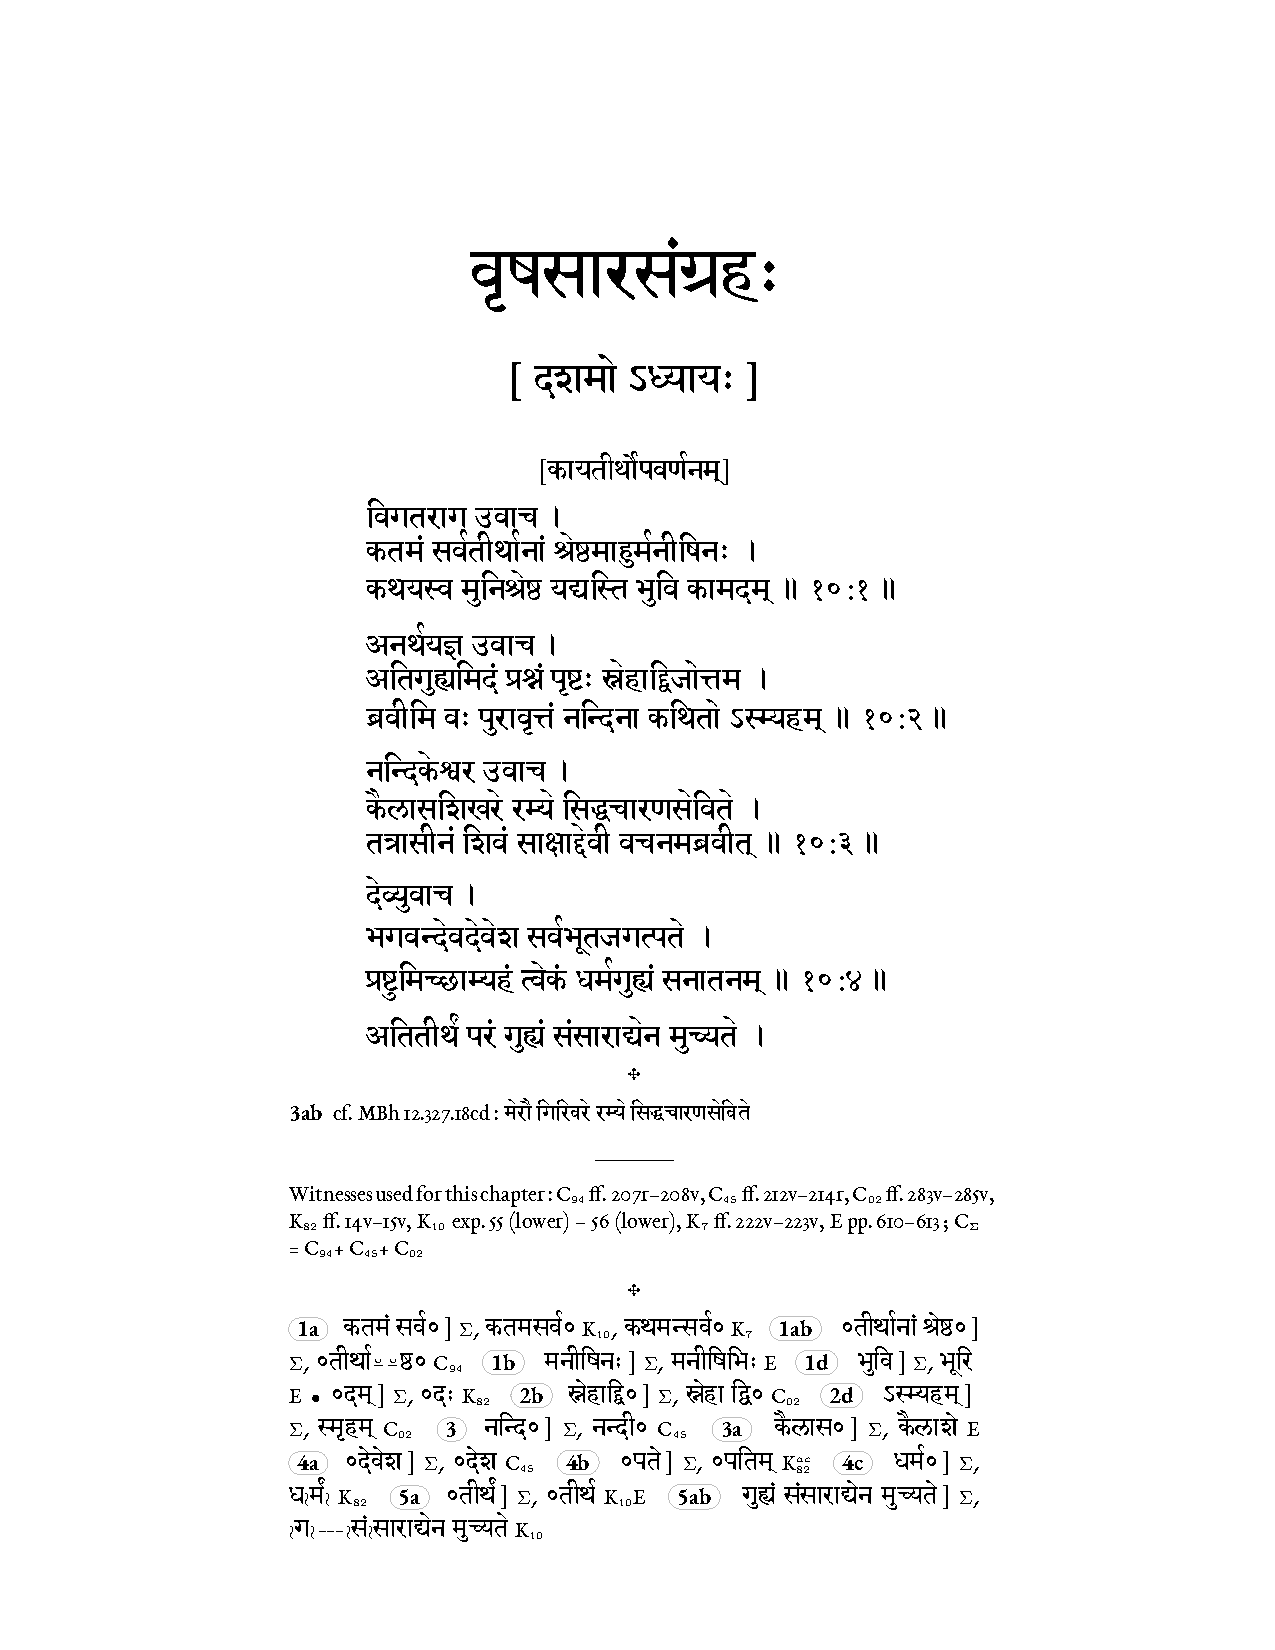
\includepdf[pages=-]{/home/csaba/indology/dharma_project/vrsa_edition/vrsasara_ed_devnag_xelatex.pdf}



%\mychapter{Notes on the Constituted Text}{notes-on-the-constituted-text}



\mychapter{An Annotated Translation}


\fancyhead[CO]{{\footnotesize \textit{Vṛṣasārasaṃgraha}}}
\fancyhead[CE]{{\footnotesize \textit{Translation of chapter 1}}}
%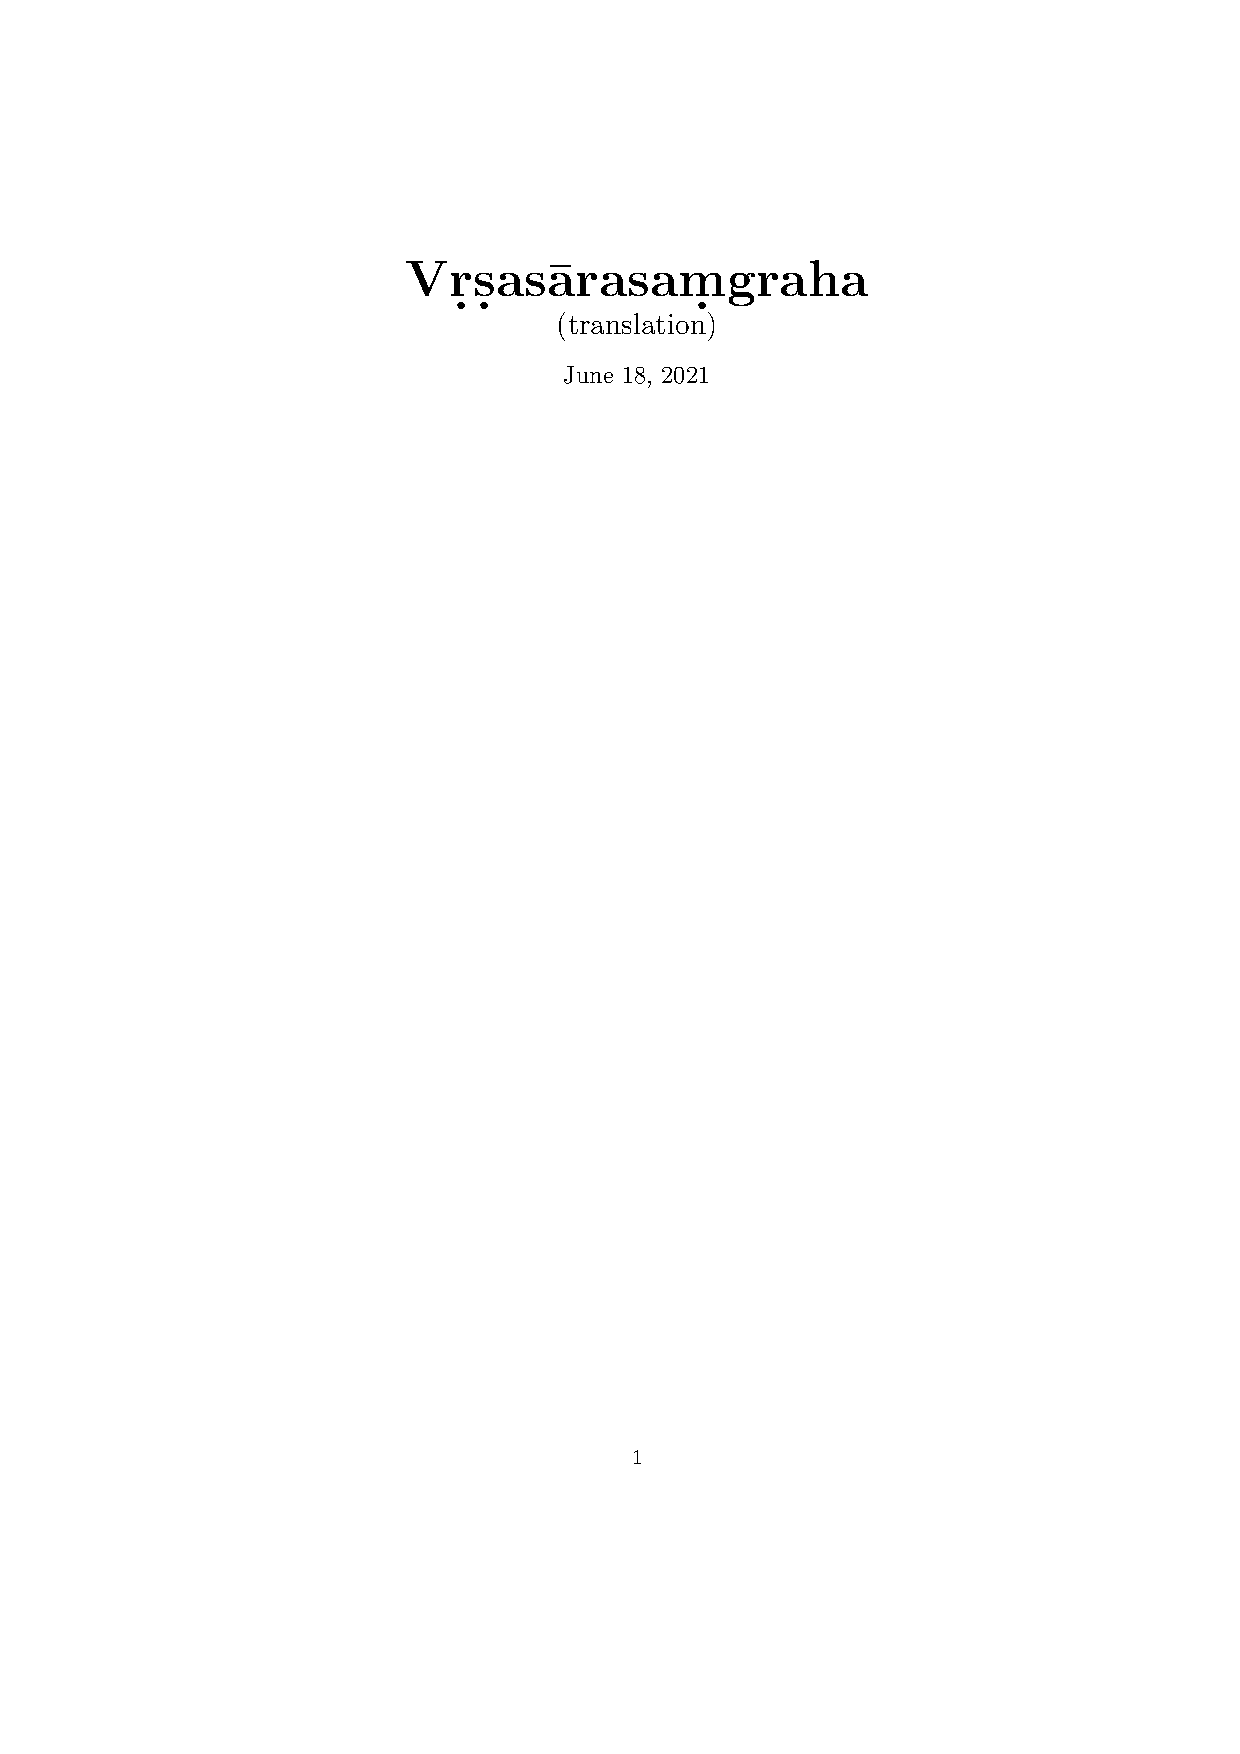
\includepdf[pages=-]{/home/csaba/indology/dharma_project/vrsa_edition/vss_translation.pdf}

% CORRECT PAGE NUMBER AFTER SKT EDITION !
\setcounter{page}{1000}
% !TEX TS-program = xelatex
% !TEX encoding = UTF-8

% This is a simple template for a XeLaTeX document using the "article" class,
% with the fontspec package to easily select fonts.

\documentclass[11pt]{article} % use larger type; default would be 10pt

\usepackage{fontspec} % Font selection for XeLaTeX; see fontspec.pdf for documentation
\defaultfontfeatures{Mapping=tex-text} % to support TeX conventions like ``---''
\usepackage{xunicode} % Unicode support for LaTeX character names (accents, European chars, etc)
\usepackage{xltxtra} % Extra customizations for XeLaTeX

\setmainfont{Ariel} % set the main body font (\textrm), assumes Charis SIL is installed
%\setsansfont{Deja Vu Sans}
%\setmonofont{Deja Vu Mono}

% other LaTeX packages.....
\usepackage[width=12cm]{geometry} % See geometry.pdf to learn the layout options. There are lots.
\geometry{a4paper} % or letterpaper (US) or a5paper or....
%\usepackage[parfill]{parskip} % Activate to begin paragraphs with an empty line rather than an indent

\usepackage{graphicx} % support the \includegraphics command and options


\begin{document}

\textit{Qualities}

\end{document}










\chapter*{Appendices}
\addcontentsline{toc}{chapter}{\hspace{1.4em}Appendices}

\thispagestyle{empty}
passeges from part two

\vfill
\pagebreak







\chapter*{Abbreviations and Bibliography}
\addcontentsline{toc}{chapter}{\hspace{1.4em}Abbreviations and Bibliography}

\begin{itemize}

\item
  CUL = Cambridge University Library 
\end{itemize}

\ldots{} TO BE SUPPLIED

\begin{itemize}
\item
  Balogh 2018? ON THE SAME TOPIC
\item
  Ranjan Sen 2006. `Vowel-weakening before muta cum liquidā sequences in
  Latin. A problem of syllabification?' In: Oxford University Working
  Papers in Linguistics, Philology \& Phonetics 11: 143-61.
\end{itemize}

% \textenglish ends



\vfill
\pagebreak

\noindent
\textsanskrit{\large 
%तपःस्वाध्यायनिरतं तपस्वी वाग्विदां वरम् ।\\
%नारदं परिपप्रच्छ वाल्मीकिर्मुनिपुंगवम् ॥\\
%को ऽन्वस्मिन्साम्प्रतं लोके गुणवान्कश्च वीर्यवान् ।\\
%धर्मज्ञश्च कृतज्ञश्च सत्यवाक्यो दृढव्रतः ॥ \\
%तपःस्वाध्यायनिरतं तपस्वी वाग्विदां वरम् ।\\
%नारदं परिपप्रच्छ वाल्मीकिर्मुनिपुंगवम् ॥\\
%को ऽन्वस्मिन्साम्प्रतं लोके गुणवान्कश्च वीर्यवान् ।\\
%धर्मज्ञश्च कृतज्ञश्च सत्यवाक्यो दृढव्रतः ॥ \\
%तपःस्वाध्यायनिरतं तपस्वी वाग्विदां वरम् ।\\
%नारदं परिपप्रच्छ वाल्मीकिर्मुनिपुंगवम् ॥\\
%को ऽन्वस्मिन्साम्प्रतं लोके गुणवान्कश्च वीर्यवान् ।\\
%धर्मज्ञश्च कृतज्ञश्च सत्यवाक्यो दृढव्रतः ॥ \\
%तपःस्वाध्यायनिरतं तपस्वी वाग्विदां वरम् ।\\
%नारदं परिपप्रच्छ वाल्मीकिर्मुनिपुंगवम् ॥\\
%को ऽन्वस्मिन्साम्प्रतं लोके गुणवान्कश्च वीर्यवान् ।\\
%धर्मज्ञश्च कृतज्ञश्च सत्यवाक्यो दृढव्रतः ॥ 
}

%(\cite[see][13 ff.]{OlivelleGrhastha})






% print biblio:
\bibliographystyle{csaba2022}
%\renewcommand*{\bibname}{References huhu}
\label{bibliography}
\bibliography{vssbiblio}
\addcontentsline{toc}{chapter}{\hspace{1.4em}REFFFS!}






\label{index}
\renewcommand*{\indexname}{{\normalfont Index}}
\printindex

\listoftodos


\end{document}
